\section{Codes to Improve Accesses}
\label{sec:code_design}

%In this section, we discuss one of the main components of the memory design proposed in this paper. 
Introducing redundancy into a storage space comprised of single-port memory banks enables simultaneous memory access. In this section we propose memory designs that utilize coding schemes which are designed for access-efficiency. We first define some basic concepts with an illustrative example and then describe $3$ coding schemes in detail.

\begin{comment}
Coding theory is the study of codes and their applications  to specific fields.  
Coding has been used in a variety of computer  science applications,  from error 
correction in the transmission of data  to increased compression for data  
storage.  We aim to extend the benefits of coding theory  to improve the 
efficiency of random-access  memory systems.  We propose a memory scheme in 
which a small portion of memory is reserved for the efficient coding of 
pre-existing data.  In essence, this allows the data of one bank to be 
duplicated and stored in an additional memory location.  Traditionally, when 
multiple  requests  to a single bank  are issued by the processor, a stall is 
generated.  These types of stalls, known as bank conflicts, result from the fact 
that  only one address from a single bank can be accessed at a time.  The 
processor must wait for the result from the first bank access to return  before 
it can serve additional  requests to the same bank.  This lag can be a major 
bottleneck in a computer's processing speed. With a coded memory scheme, data 
present in multiple data banks will be compressed and stored in extra banks, 
known as a parity banks.  These parity banks will then be accessed concurrently 
with corresponding data  banks to help alleviate stalls from bank conflicts.  
Ultimately,  with the addition  of a single parity  bank we are able to generate 
a single additional  access to any arbitrary bank  without  implementing  any 
further  logic to the bank  itself.  In the following sections, we first 
describe the design parameters used to design the coding system.  We then 
describe each of the three code schemes explored in this project.
\end{comment}

\subsection{Coding for memory banks}
\label{sec:coding_mb}

A coding scheme defines how memory is encoded to yield redundant storage. The memory structures which store the original memory elements are known as {\em data banks}. The elements of the data banks go through an {\em encoding process} which generates a number of {\em parity banks}.  The parity banks contain elements constructed from elements drawn from two or more data banks. A linear encoding process such as XOR may be used to minimize computational complexity. The following example further clarifies these concepts and provides some necessary notation.

\begin{example}
Consider a setup with two data banks $\mathbf{a}$ and $\mathbf{b}$. We assume that each of the banks store $L \cdot W$ binary data elements\footnote{It is possible to work with data elements over larger alphabets/finite fields. However, assuming data elements to be binary suffices for this paper as only work with coding schemes defined over binary field.} which are arranged in an $L \times W$ array. In particular, for $i \in [L] \triangleq \{1,\ldots, L\}$, $a(i)$ and $b(i)$ denote the $i$-th row of the bank $\mathbf{a}$ and bank $\mathbf{b}$, respectively. Moreover, for $i \in [L]$ and $j \in [W] \triangleq \{1,\ldots, W\}$, we use $a_{i, j}$ and $b_{i, j}$ to denote the $j$-th element in the rows $a(i)$ and $b(i)$, respectively. Therefore, for $i \in [L]$, we have 
\begin{align}
a(i) = \big(a_{i,1}, a_{i,2},\ldots, a_{i, W}\big) \in \{0, 1\}^W\nonumber \\
b(i) = \big(b_{i,1}, b_{i,2},\ldots, b_{i, W}\big) \in \{0, 1\}^W. \nonumber
\end{align}
Now, consider a linear coding scheme that produces a parity bank $\mathbf{p}$ with $L'W$ bits arranged in an $L' \times W$ array such that for $i \in [L'] \triangleq \{1,\ldots, L'\}$, 
\begin{align}
p(i) &= \big(p_{i, 1},\ldots, p_{i,W}\big) = a(i) + b(i) \nonumber \\
&\triangleq \left(a_{i,1} + b_{i,1}, a_{i,1} + b_{i,1},\ldots, a_{i,1} + b_{i,1}\right). 
\end{align}
\end{example}
\begin{remark}
Figure~\ref{fig:example1} illustrates this coding scheme. Because the parity bank is based on those rows of the data banks that are indexed by the set $[L'] \subseteq [L]$, we use the following concise notation to represent the encoding of the parity bank. 
$$
\mathbf{p} = \mathbf{a}([L']) +  \mathbf{b}([L']).
$$
In general, we can use any subset $\mathcal{S} = \{i_1, i_2,\ldots, i_{L'}\} \subseteq [L]$ comprising $L'$ rows of data banks to generate the parity bank $\mathbf{p}$. In this case, we have $\mathbf{p} = \mathbf{a}(\mathcal{S}) +  \mathbf{b}(\mathcal{S})$, or
\begin{align*}
p(l) = a(i_l) + b(i_l)~\text{for}~l \in [L'].
\end{align*}
%Figure~\ref{fig:example1_case2} illustrates the case with a generic set $\mathcal{S}$.% $ = [L - L'  + 1,\ldots, L]$.
\end{remark}

%%%%%%%%%%%%%%%%%%%%%%%%%%%%%%%%%%%
%\begin{figure}[t!]
%\centering
%\begin{subfigure}[b]{0.48\linewidth}
%  \centering
%  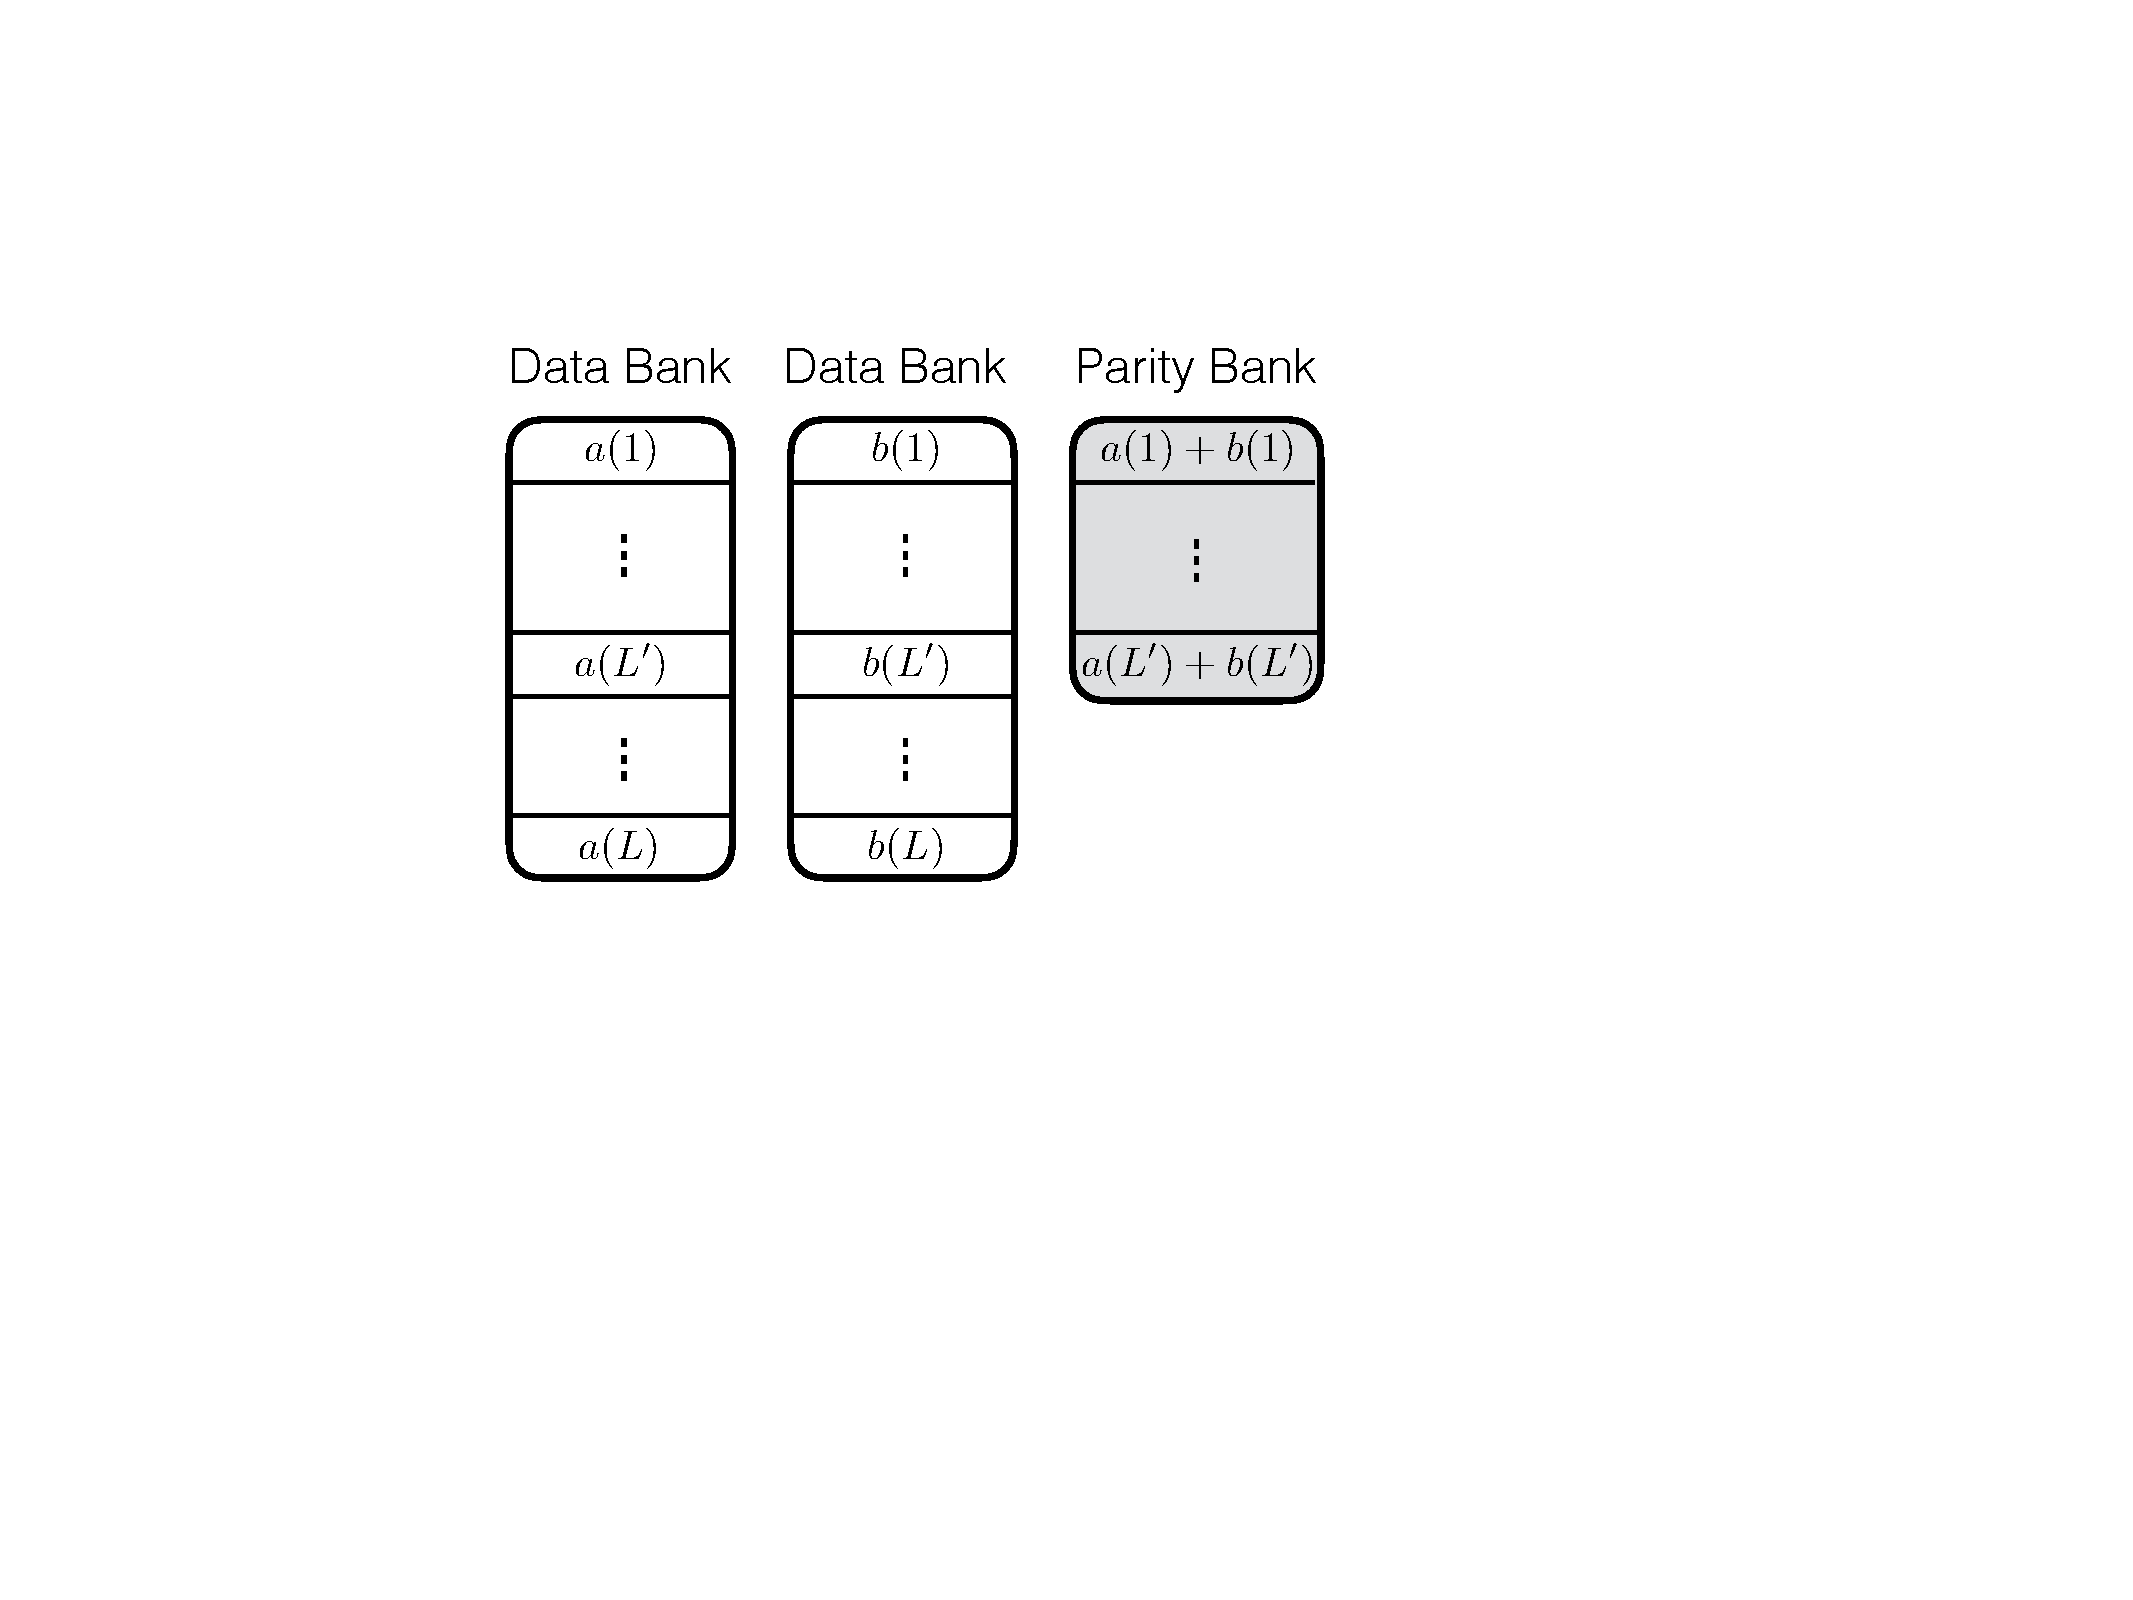
\includegraphics[width=0.95\linewidth]{fig/example-inter-bank.pdf} 
%  \caption{{\color{red}Parity.}}
%  \label{fig:example1_case1}
%\end{subfigure}
%\begin{subfigure}[b]{0.48\linewidth}
%  \centering
%  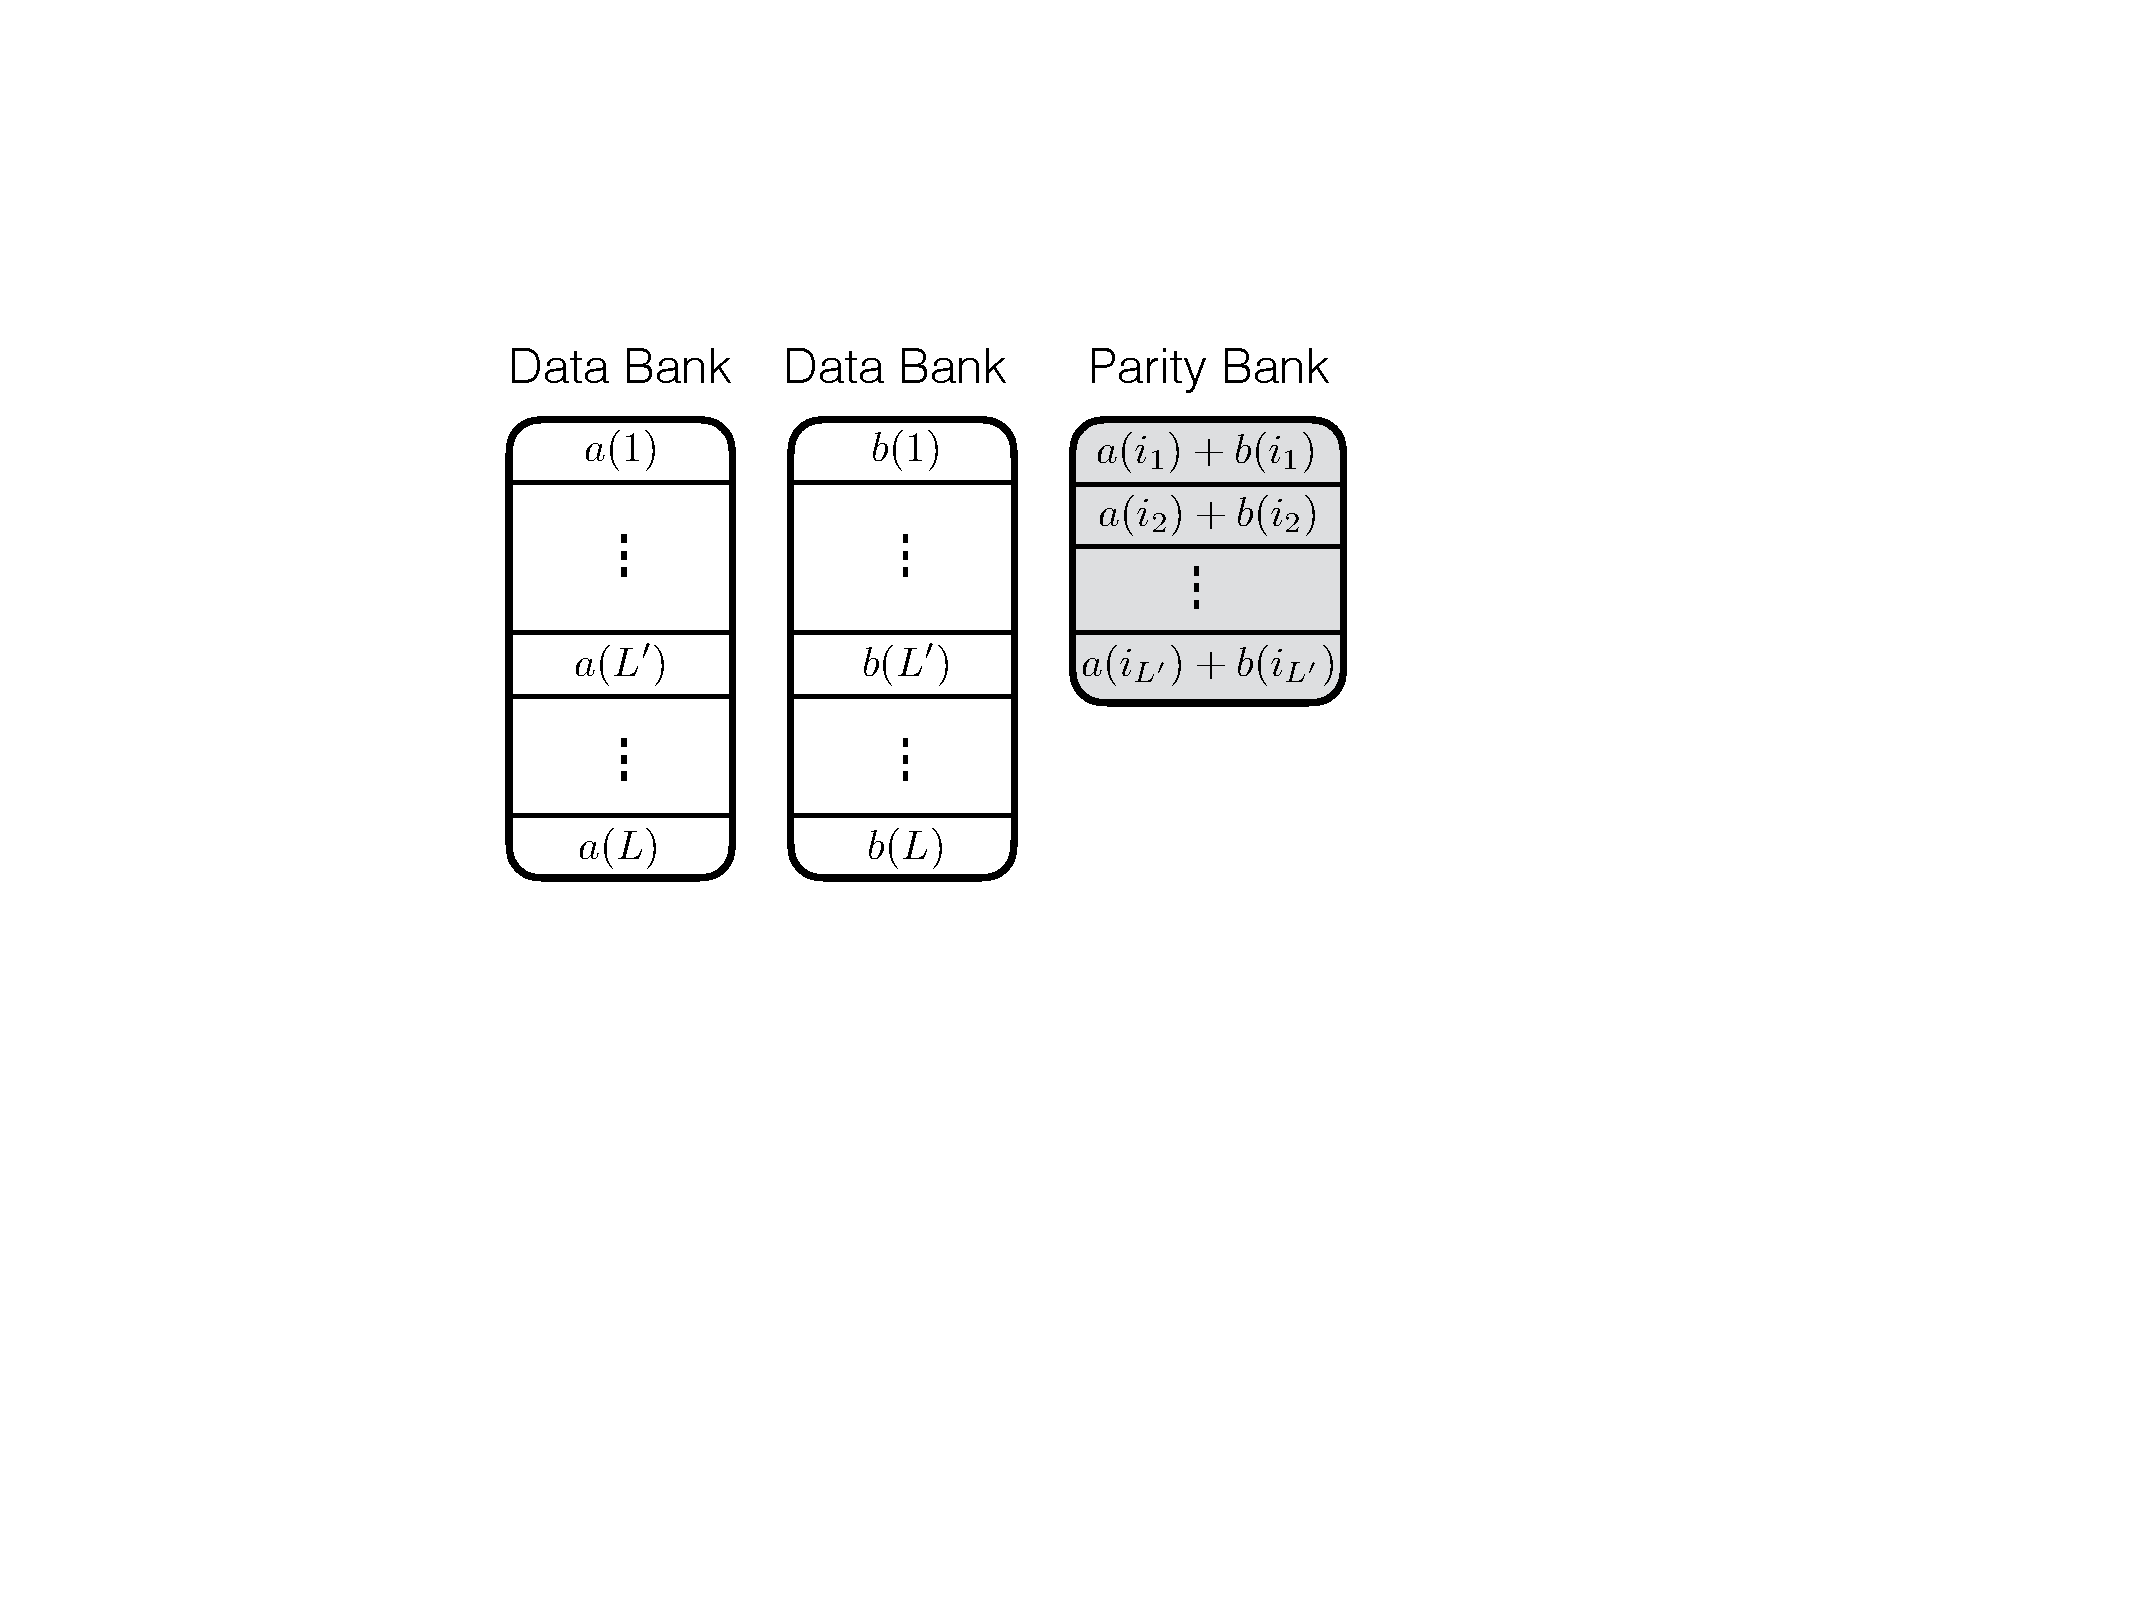
\includegraphics[width=0.98\linewidth]{fig/example-inter-bank-2.pdf} 
%  \caption{{\color{red}Parity.}}
%  \label{fig:example1_case2}
%\end{subfigure}
%\caption{{\color{red}Design.}}
%\label{fig:example1}
%\end{figure}
\begin{figure}[t!]
\centering
  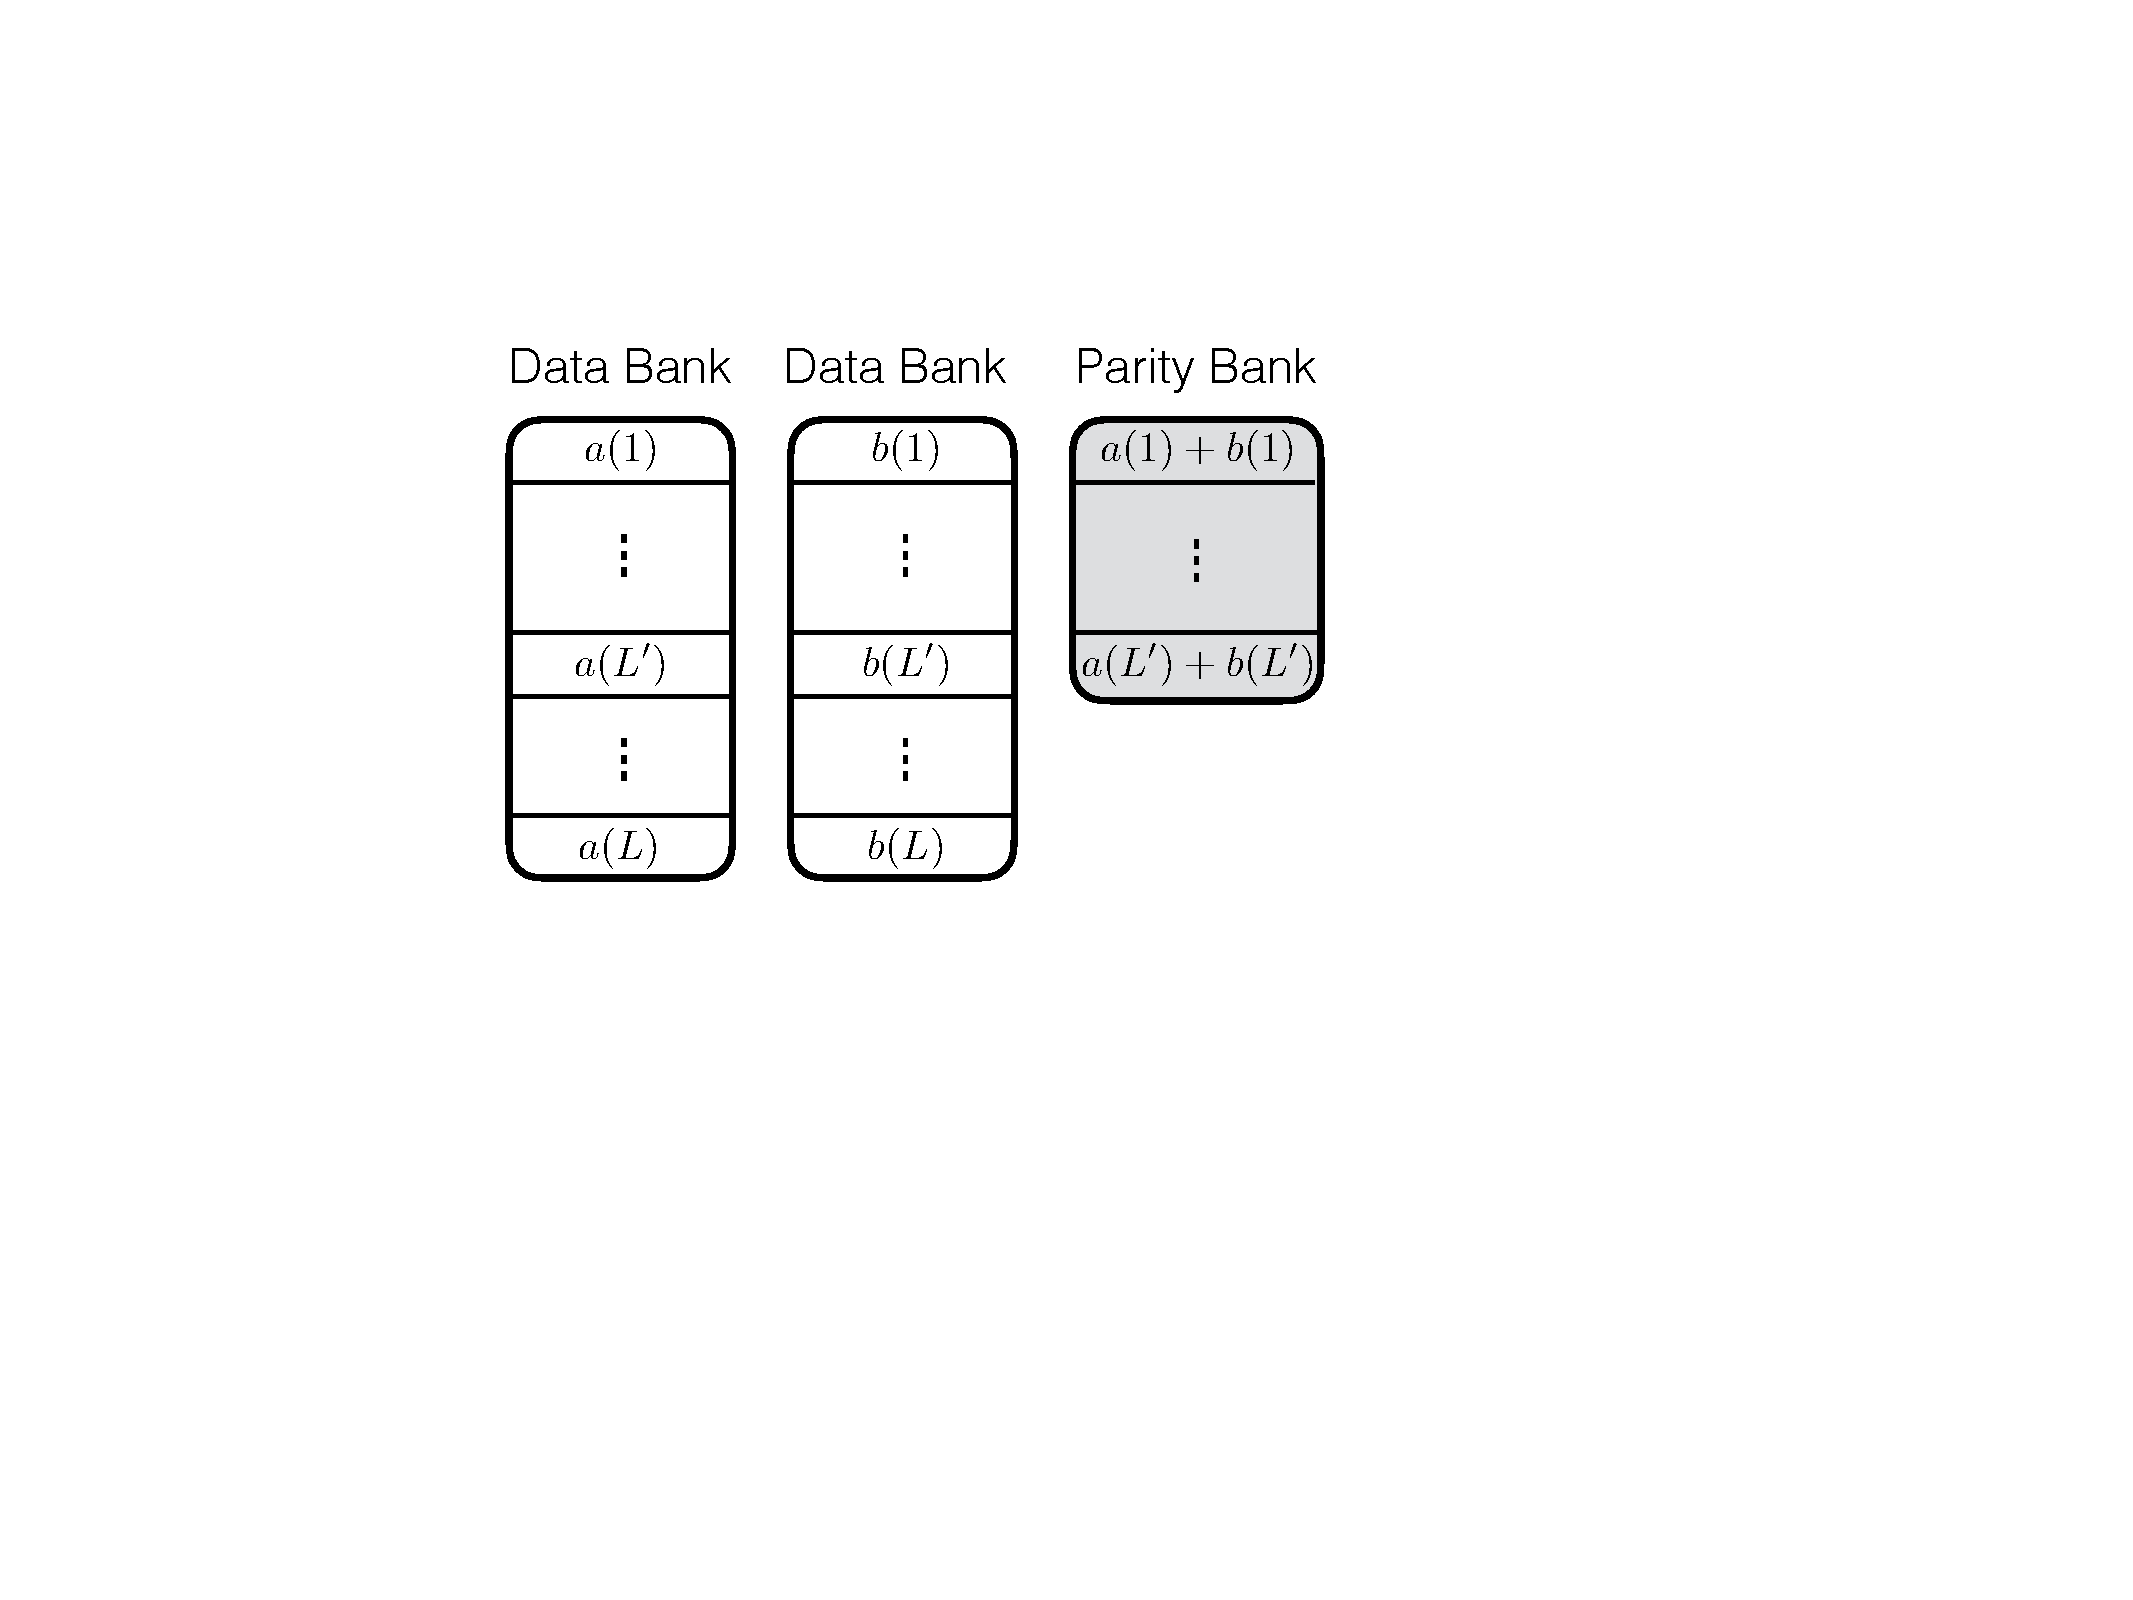
\includegraphics[width=0.45\linewidth]{fig/example-inter-bank.pdf} 
\caption{\it{This illustration is an example parity design.}}
\label{fig:example1}
\end{figure}
%%%%%%%%%%%%%%%%%%%%%%%%%%%%%%%%%%%%%%


\begin{remark}
Note that we allow for the data banks and parity banks to have different sizes, \textit{i.e.} $L \neq L'$. This freedom in memory design can be utilized to reduce the storage overhead of parity banks based on the underlying application. If the size of a parity bank is smaller than a data bank, \textit{i.e.} $L' < L$, we say that the parity bank is a {\em shallow bank}. We note that it is reasonable to assume the existence of shallow banks, especially in proprietary designs of integrated memories in a system on a chip (SoC).
\end{remark}

\begin{remark}
\label{rem:design1}
Note that the size of shallow banks is a design choice which is controlled by the parameter $0 < \alpha \leq 1$. A small value of $\alpha$ corresponds to small storage overhead. The choice of a small $\alpha$ comes at the cost of limiting parity memory accesses to certain memory ranges. In Section~\ref{sec:dynamicCoding} we discuss techniques for choosing which regions of memory to encode. In scenarios where many memory accesses are localized to small regions of memory, shallow banks can support many parallel memory accesses for little storage overhead. For applications where memory access patterns are less concentrated, the robustness of the parity banks allows one to employ a design with $\alpha = 1$.
\end{remark}

\subsubsection{Degraded reads and their locality}
\label{sec:degraded}

The redundant data generated by a coding scheme mitigates bank conflicts by supporting multiple read accesses to the original data elements. Consider the coding scheme illustrated in Figure~\ref{fig:example1} with a parity bank $\mathbf{p} = \mathbf{a}([L']) + \mathbf{b}([L'])$. In an uncoded memory system simultaneous read requests for bank $\mathbf{a}$, such as $a(1)$ and $a(5)$, result in a bank conflict. The introduction of $\mathbf{p}$ allows both read requests to be served. First, $a(1)$ is served directly from bank  $\mathbf{a}$. Next, $b(5)$ and $p(5)$ are downloaded. $a(5) = b(5) + p(5)$, so $a(5)$ is recovered by means of the memory in the parity bank. A read request which is served with the help of parity banks is called a {\em degraded read}. Each degraded read has a parameter {\em locality} associated with it which corresponds to the total number of banks used to serve it. In this case, the degraded read for $a(5)$ using $\mathbf{b}$ and $\mathbf{p}$ has locality $2$.

%In order to further illustrate the notion of locality, let's consider a setup where we generate a parity bank $\mathbf{p}$ by combining three data banks $\mathbf{a}$, $\mathbf{b}$, and $\mathbf{c}$ as $\mathbf{p} = \mathbf{a} + \mathbf{b} + \mathbf{c}$. Now, a degraded read for $a(1)$ using the parity bank as $$a(1) = b(1) + c(1) + p(1) = b(1) + c(1) + \big(a(1) + b(1) + c(1)\big)$$
%has locality $3$ as the degraded read is served using three memory banks.

\subsection{Codes to emulate multi-port memory}
\label{sec:designs}

We will now describe the code schemes proposed for the emulation of multi-port memories. Among a large set of possible coding schemes, we focus on three specific coding schemes for this task. We believe that these three coding schemes strike a good balance among various quantitative parameters, including storage overhead, number of simultaneous read requests supported by the array of banks, and the locality associated with various degraded reads. Furthermore, these coding schemes respect the practical constraint of encoding across a small number of data banks. In particular, we focus on the setup with $8$ memory banks, which contrasts with communications applications where encoding typically occurs with blocks of $1024$ or more information symbols. 

In the rest of this section, we present three code schemes and discuss the number of simultaneous read requests supported by these schemes in the best and worst case. We summarize all the relevant parameters associated with these schemes in Table~\ref{table:codedesigncomparison}.
%
%We discuss the design of the codes for creating extra accesses to memory in this 
%section. First we discuss the code schemes explored during Phase I. Second, we discuss 
%specific execution strategies to efficiently implement the designs.\\
%In the following sub-sections, we discuss 3 designs for storing coded data.  
%Table~\ref{table:codedesigncomparison} compares these designs for various 
%parameters and associated costs.  
%\begin{table*}[t]
%\centering
%	\begin{tabular}{|m{1cm}|m{2 cm}|m{1cm}|m{1cm}|m{1cm}|m{1cm}|m{1cm}|}
%\hline
%Design & Max Read per bank & Max Write per bank & Locality & Rate & Memory 
%Overhead & Logical Complexity \\ \hline
%I & 4 & 2 & 2 & $2/5$ & 1.5 $\alpha$ & Low \\ \hline
%II & 5 & 2 & 2 & $2/5$ & 2.5 $\alpha$ & Medium \\ \hline
%III & 4 & 2 & 3 & $1/2$ & \text{      } $\alpha$ & Medium \\ \hline
%	\end{tabular}
%	\caption{Comparison of design with respect to the performance parameters 
%	and associated cost}
%	\label{table:codedesigncomparison}
%\end{table*}


%\begin{tiny}
%\begin{table}[t!]
%  \centering
%  \begin{tabular}{|c|c|c|c|c|c|c|}
%    \hline
%    \textbf{Design} & \textbf{Max reads} & \textbf{Max writes} & \textbf{Locality} & \textbf{Rate} & \textbf{Storage overhead} & \textbf{Logical complexity} \\
%    & \textbf{(per bank)} & \textbf{(per bank)} & & & & \\
%    \hline
%    \hline
%    I & 4 & 2 & 2 & $2/5$ & 1.5 $\alpha$ & Low \\ \hline
%II & 5 & 2 & 2 & $2/5$ & 2.5 $\alpha$ & Medium \\ \hline
%III & 4 & 2 & 3 & $1/2$ & \text{      } $\alpha$ & Medium \\ 
%\hline                                   
%  \end{tabular}
%	\caption{Comparison of the code schemes with respect to the performance parameters and associated cost}
%	\label{table:codedesigncomparison}
%\end{table}
%\end{tiny}

\begin{comment}
\begin{table}[t!]
  \centering
  \begin{tabular}{|c|c|c|c|c|c|}
    \hline
   {\small Design} & {\small  Max reads} &{\small  Locality} & {\small  Rate} & {\small  Storage} & {\small  Logical } \\
    & {\small  (per bank)} & & &{\small  overhead} & {\small  complexity} \\
    \hline
    \hline
    {\small I} & {\small$4$ } & {\small$2$} & {\small ${2}/{5}$} & {\small $1.5\alpha$} & {\small Low} \\ \hline
{\small II} & {\small$5$}  & {\small$2$} & {\small ${2}/{5}$} & {\small $2.5\alpha$} & {\small Medium} \\ \hline
{\small III }& {\small$4$}  & {\small$3$} & {\small$1/2$} & {\small $\alpha$} & {\small Medium} \\ 
\hline                                   
  \end{tabular}
	\caption{\it{Comparison of the code schemes with respect to the performance parameters and associated cost. $\alpha$ is the fraction of storage overhead in comparison to the data bank. $\alpha = 1$ when size of parity bank is equal to size of data bank.}}
	\label{table:codedesigncomparison}
\end{table}
\end{comment}

\begin{table}[ht!]
  \centering
  \begin{tabular}{|c|c|c|c|c|c|}
    \hline
   {\scriptsize Design} & {\scriptsize  Max reads} &{\scriptsize  Locality} & {\scriptsize  Rate} & {\scriptsize  Storage} & {\scriptsize  Logical } \\
    & {\scriptsize  (per bank)} & & {\scriptsize ($\alpha=1$)}&{\scriptsize  overhead} & {\scriptsize  complexity} \\
    \hline
    \hline
    {\scriptsize I} & {\scriptsize$4$} & {\scriptsize$2$} & {\scriptsize $\nicefrac{2}{5}$} & {\scriptsize $1.5\alpha$} & {\scriptsize Low} \\ \hline
%{\scriptsize II} & {\scriptsize$5$}  & {\scriptsize$2$} & {\scriptsize ${2}/{5}$} & {\scriptsize $2.5\alpha$} & {\scriptsize Medium} \\ \hline
{\scriptsize II} & {\scriptsize$5$}  & {\scriptsize$2$} & {\scriptsize $\nicefrac{2}{7}$} & {\scriptsize $2.5\alpha$} & {\scriptsize Medium} \\ \hline
{\scriptsize III }& {\scriptsize$4$}  & {\scriptsize$3$} & {\scriptsize$\nicefrac{1}{2}$} & {\scriptsize $\alpha$} & {\scriptsize Medium} \\ 
\hline                                   
  \end{tabular}
	\caption{\it{Comparison of the code schemes with respect to the performance parameters and associated cost.}}
	\label{table:codedesigncomparison}
\end{table}


\subsubsection{Code Scheme I}
\label{sec:design1}

This code scheme is motivated from the concept of batch codes~\cite{batchcodes} which enables parallel access to content stored in a large scale distributed storage system.
%The coding scheme is illustrated in Figure~\ref{fig:design1}. 
The code scheme involves $8$ data banks $\{\mathbf{a}, \mathbf{b},\ldots, \mathbf{h}\}$ each of size $L$ and $12$ shallow banks each of size $L' = \alpha L$. We partition the $8$ data banks into two  groups of $4$ banks. The underlying coding scheme produces shallow parity banks by separately encoding data banks from the two groups. Figure~\ref{fig:design1} shows the resulting memory banks. The storage overhead of this schemes is $12\alpha L$ which implies the rate\footnote{The information rate is a standard measure of redundancy of a coding scheme ranging from $0$ to $1$, where $1$ corresponds to the most efficient utilization of storage space.} of the coding scheme is $$\frac{8L}{8L + 12\alpha L} = \frac{2}{2 + 3\alpha}.$$


We now analyze the number of simultaneous read requests that can be supported by this code scheme. \\
%This allows us to serve multiple accesses to the coded 
%region using the parity banks. With this scheme, we guarantee that any 4 read 
%requests to the coded region can be served at any given time. As shown in 
%figure~\ref{fig:design1}, 8 banks are divided into two regions.  Each region 
%consists of 4 banks. Each region has 6 parallel shallow  banks to store the 
%parity. The colored regions shown in the banks 1-8 are the coded region. These 
%regions are assumed to be of $\alpha $ fraction of the memory. \\

\noindent \textbf{Best case analysis:~}This code scheme achieves maximum 
performance when sequential accesses to the coded regions are issued. During the 
best case access, we can achieve up to $10$ parallel accesses to a particular coded region in one access cycle.
Consider the scenario when we receive accesses to the following $10$ rows:
\begin{align*}
&\left\{a(1),b(1),c(1),d(1),a(2),b(2),c(2),d(2),c(3),d(3)\right\} .
\end{align*}
Note that we can serve the read requests for the rows \\ $\{a(1),b(1),c(1),d(1)\}$ using the data bank $\mathbf{a}$ and the three parity banks storing $\{a(1)+b(1), b(1)+c(1),c(1)+d(1)\}$. The requests for $\{a(2),c(2),d(2)\}$ can be served by downloading $b(2)$ from the data bank $\mathbf{b}$ and $\{a(2)+d(2), b(2)+d(2),a(2)+c(2)\}$ from their respective parity banks. Lastly, in the same memory clock cycle, we can serve the requests for $\{c(3), d(3)\}$ using the data banks $\mathbf{c}$ and $\mathbf{d}$.\\
%------------------------------
\begin{figure}[ht!]
\centering
	%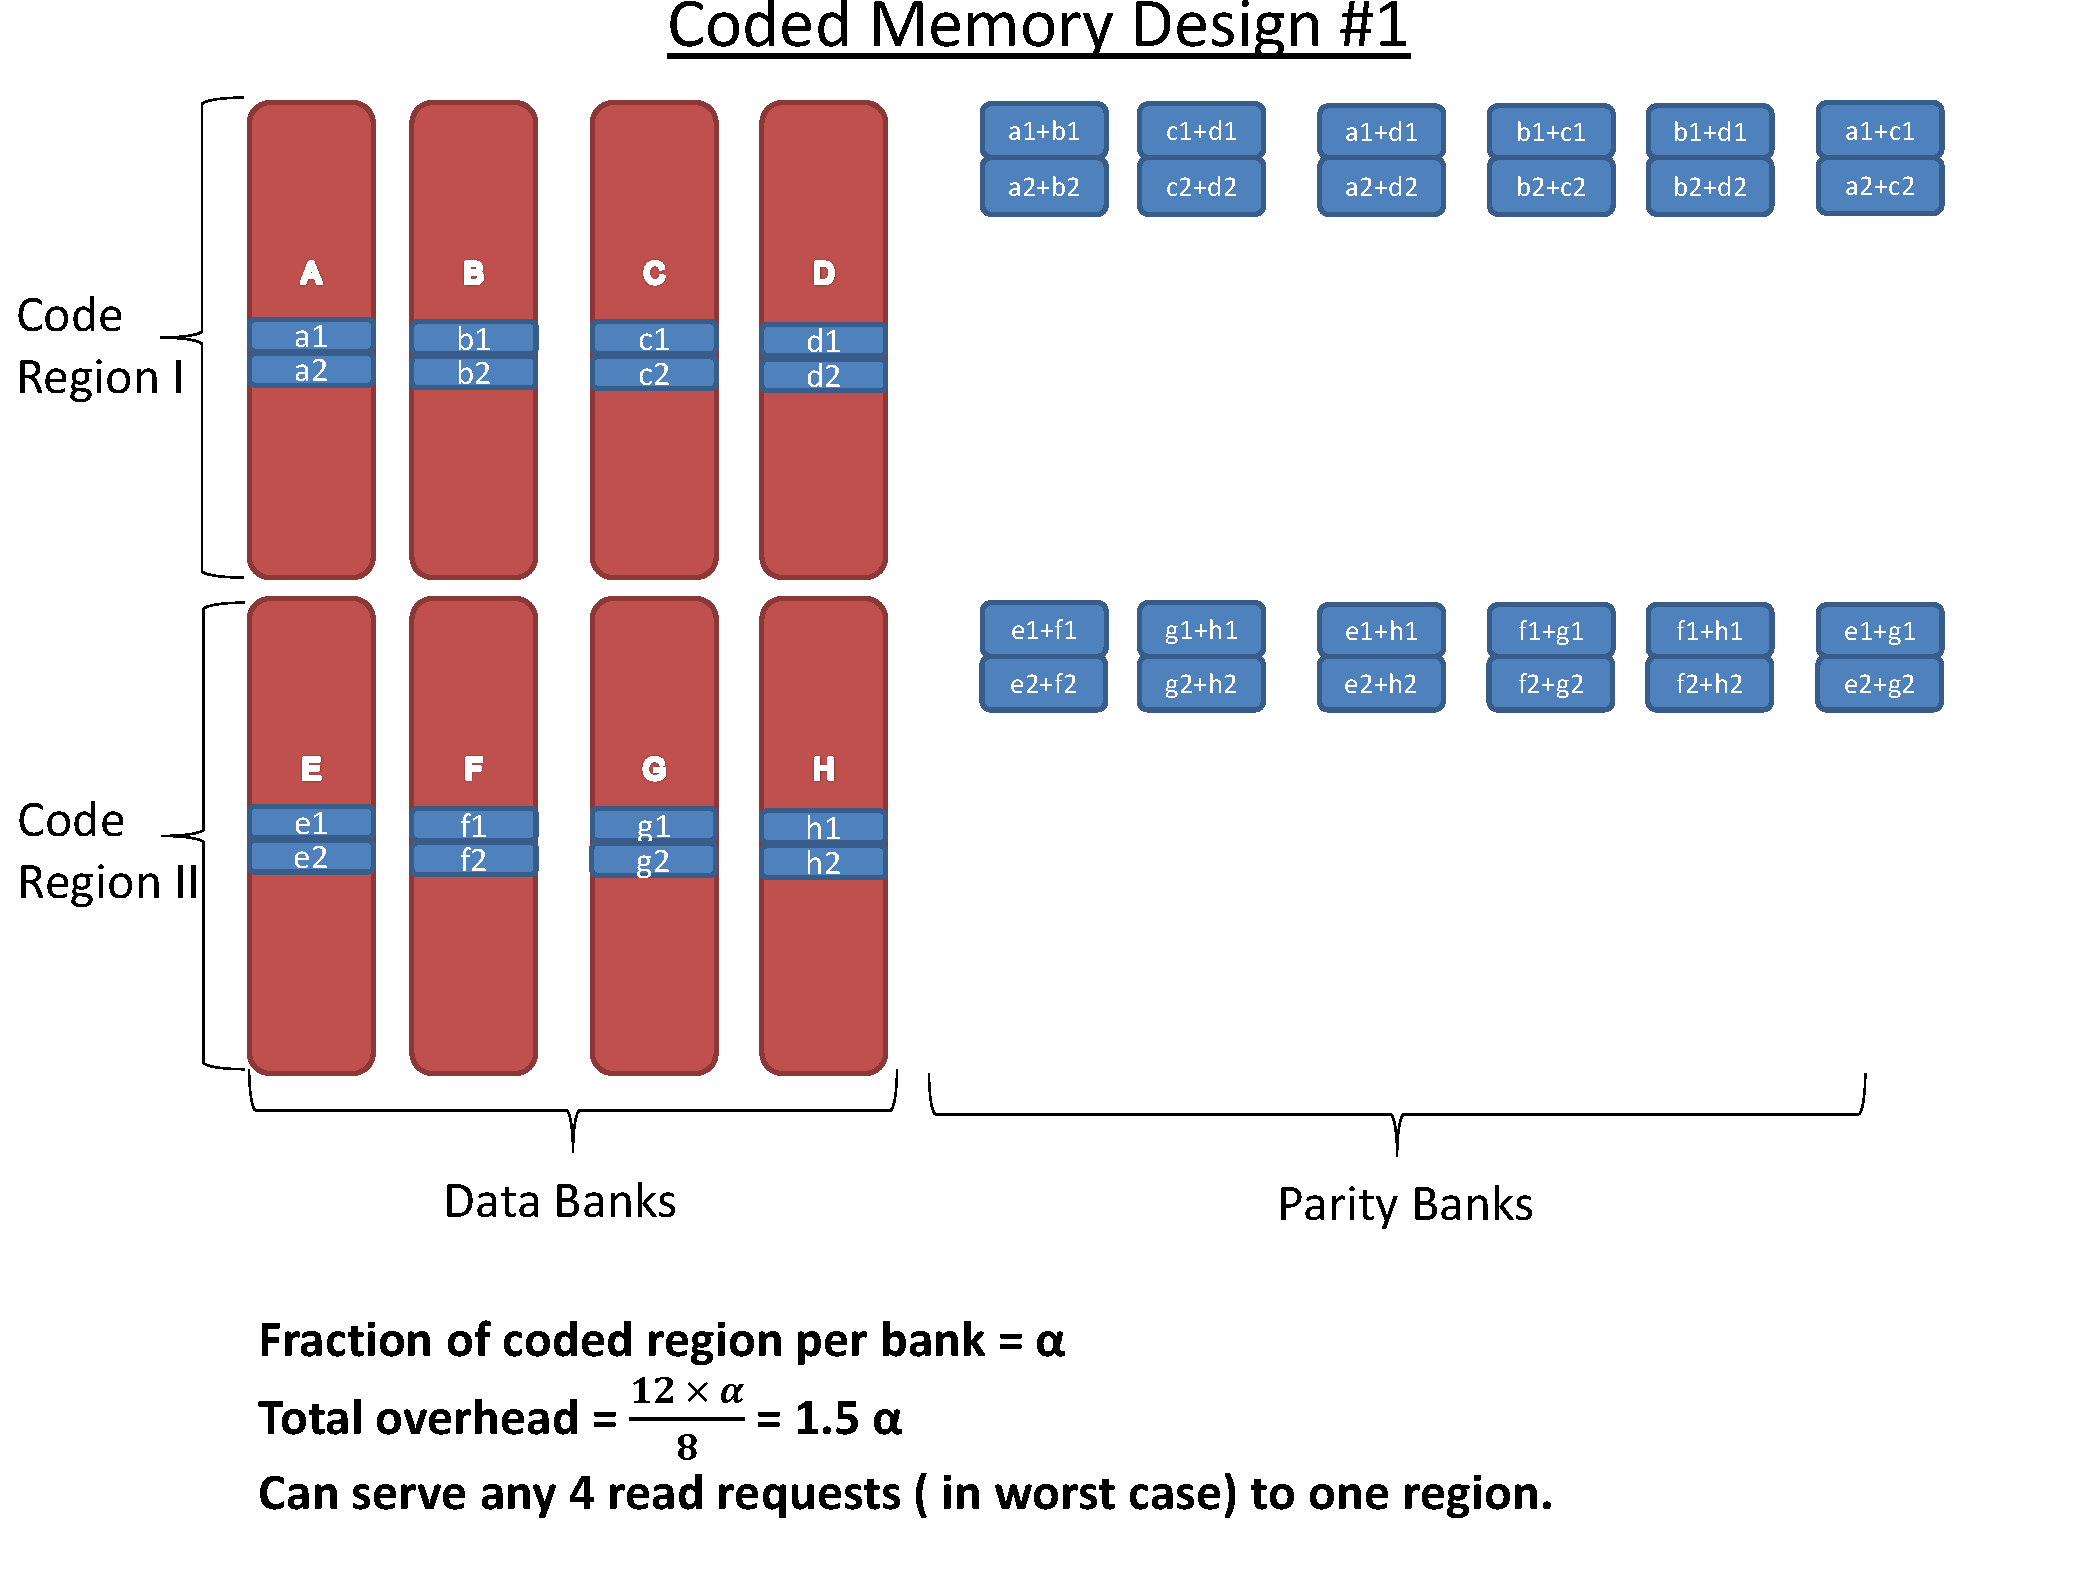
\includegraphics[width=0.8\linewidth]{fig/designI.pdf}
	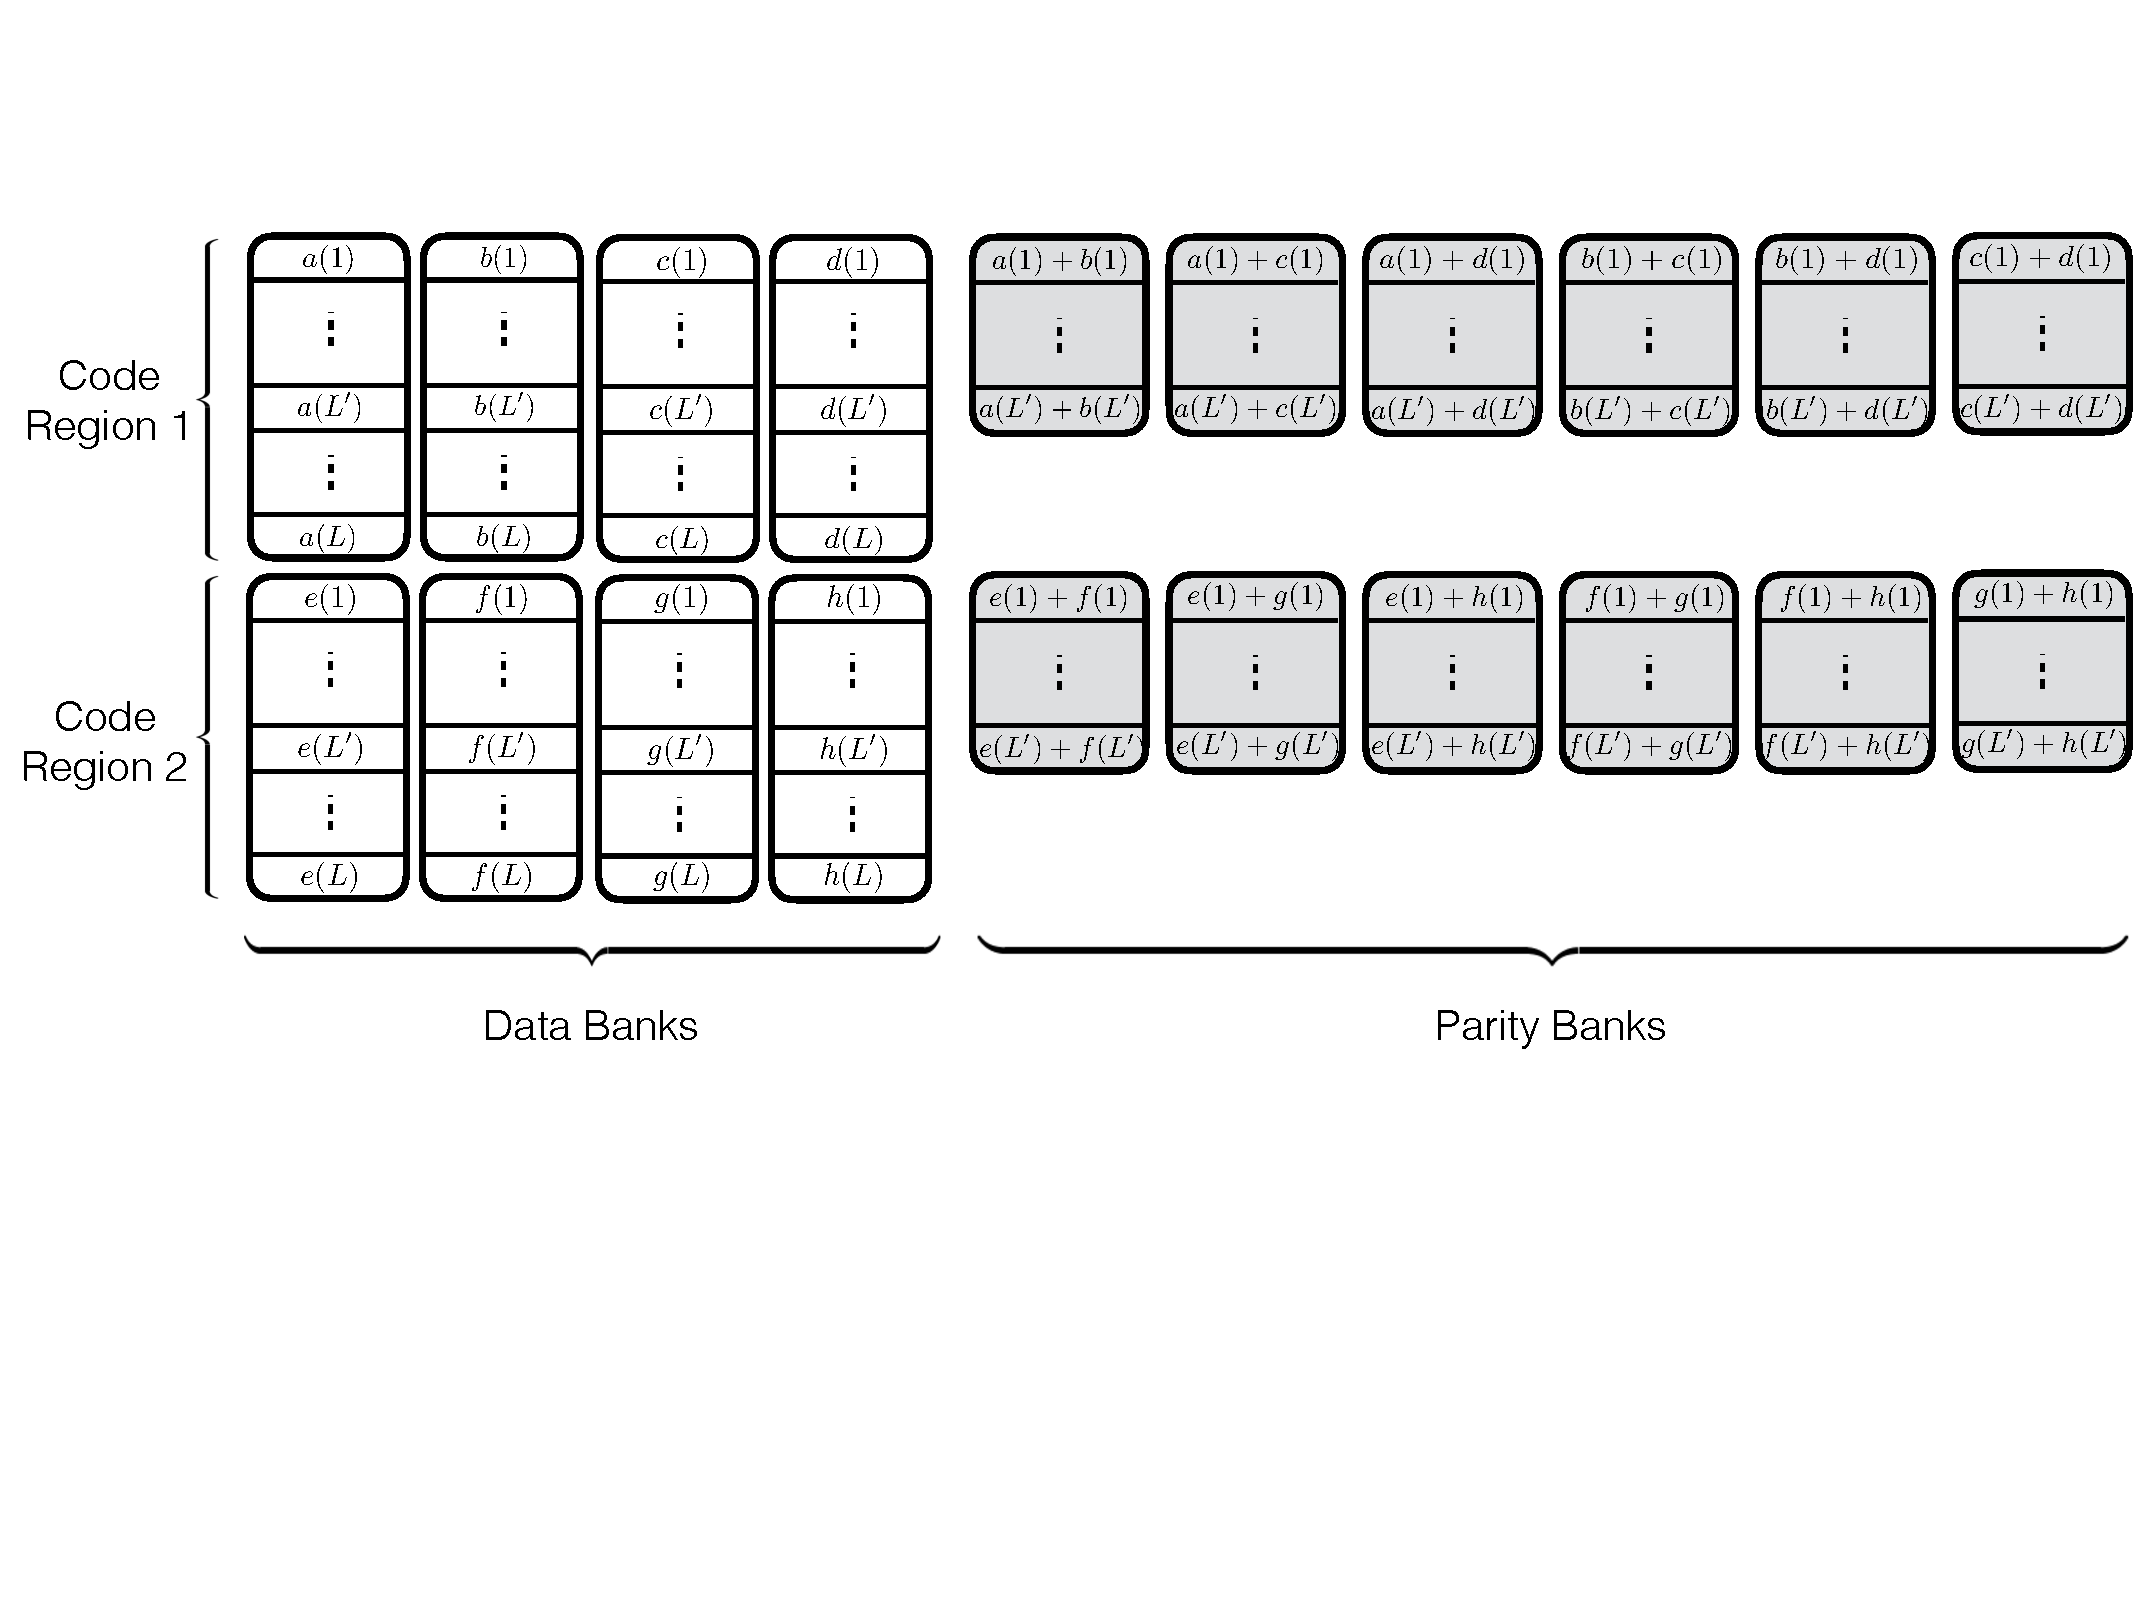
\includegraphics[width=1\linewidth]{fig/Code-Design-1.pdf}
	\caption{\it{Pictured here is an illustration of code scheme I.}}
	\label{fig:design1}
%\caption{Code Schemes}
\end{figure} 
%------------------------------
\ignore{
%------------------------------
\begin{figure}[ht!]
\centering
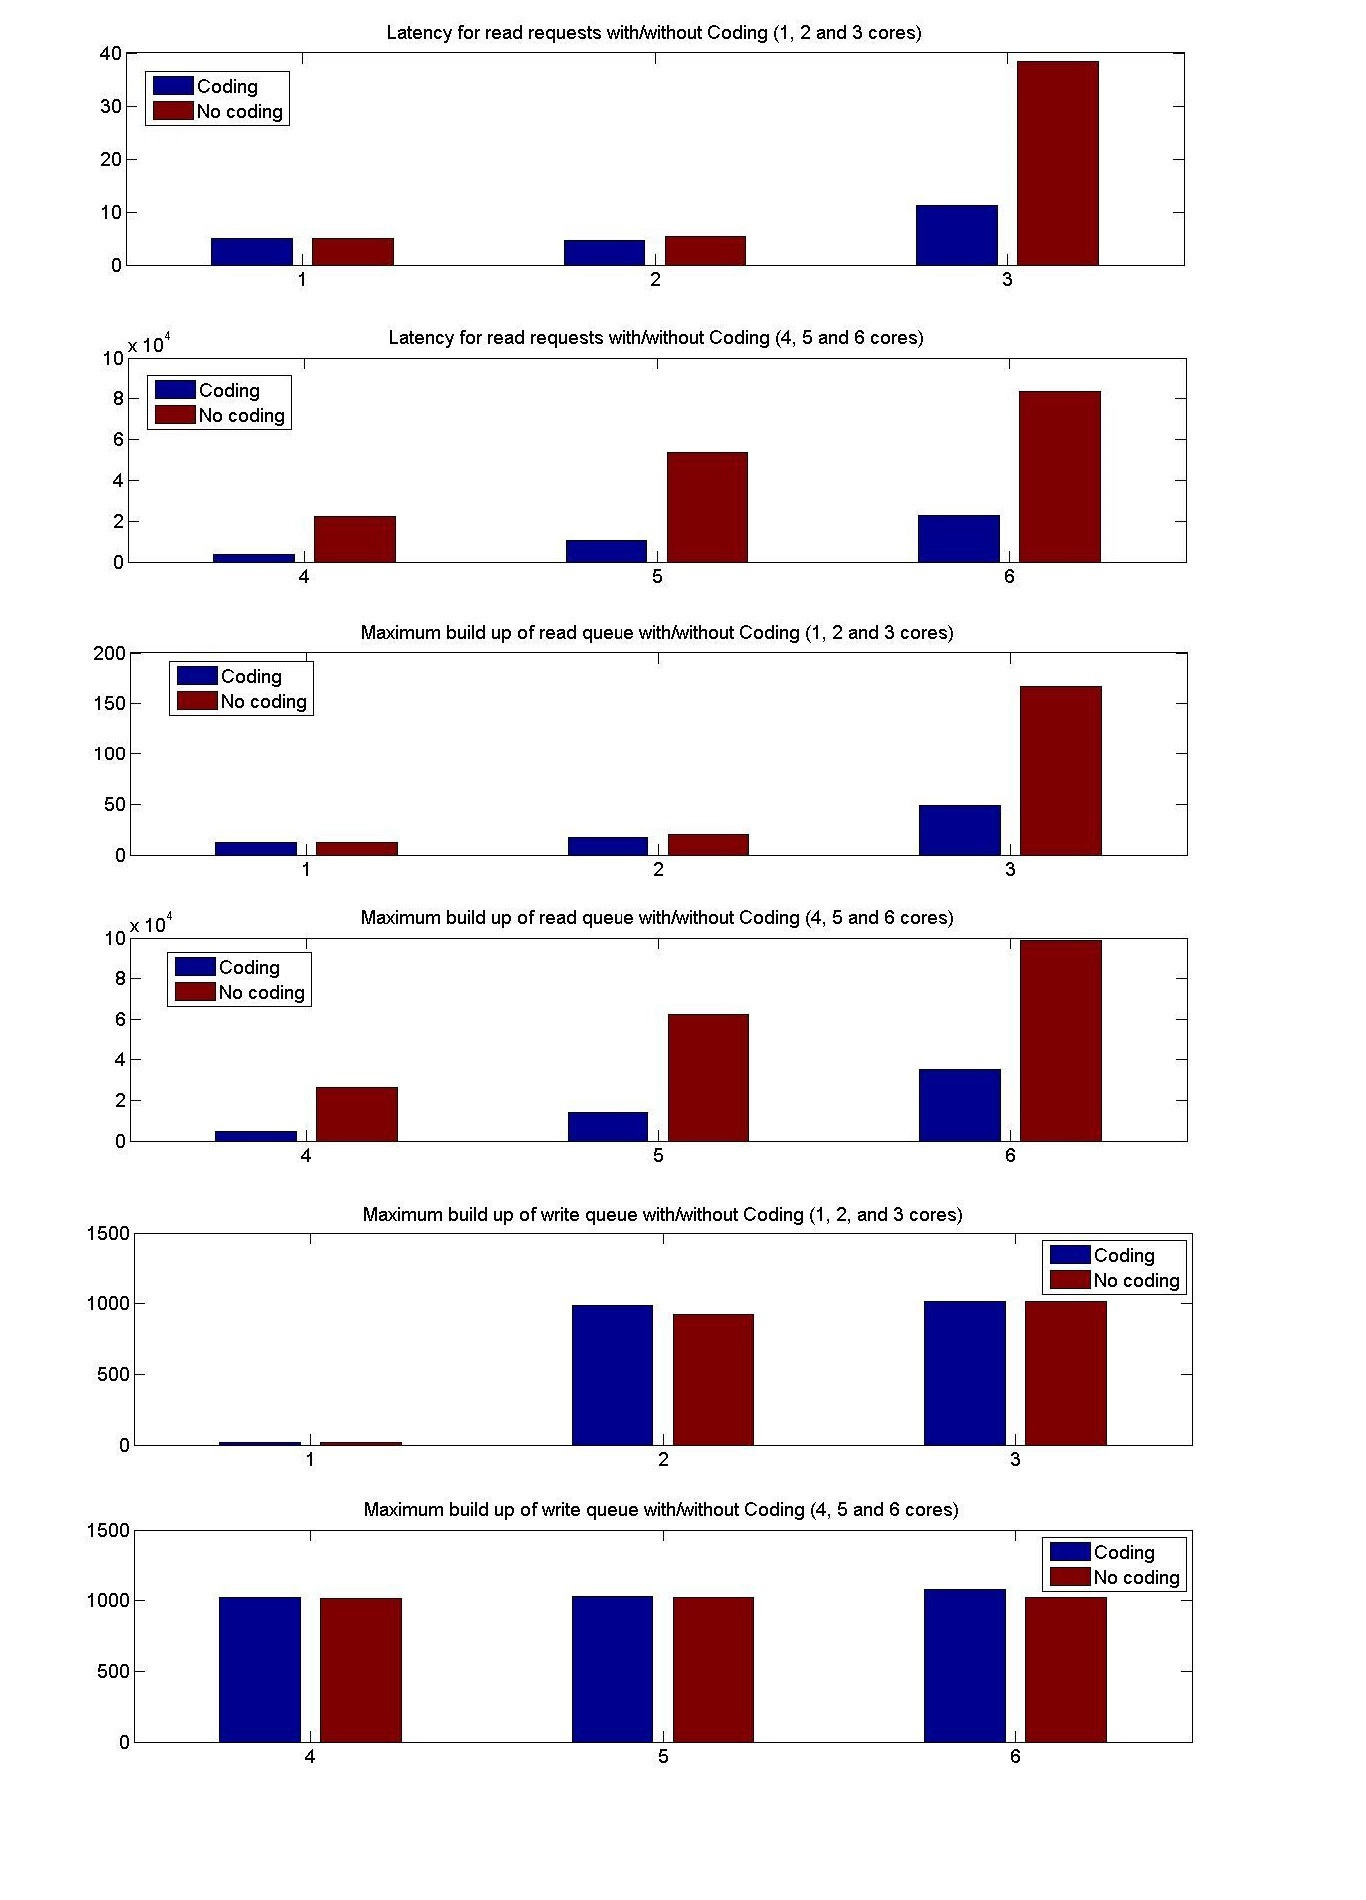
\includegraphics[width=150mm,natwidth=610,natheight=642]{fig/result_design1.jpg}
\caption{ }
\label{fig:result_design1}
\end{figure}
%------------------------------
}
\noindent \textbf{Worst case analysis}: This code scheme  (cf.~Figure~\ref{fig:design1}) may fail to utilize any parity banks depending on the requests waiting to be served. The worst case scenario for this code scheme is when there are non-sequential and non-consecutive access to the memory 
banks. Take for example a scenario where we only consider the first four banks of the code scheme. The following read requests are waiting to be served:  
\begin{align*}
\{a(1), a(2), b(8), b(9), c(10),c(11), d(14), d(15)\}. 
\end{align*}
Because none of the requests share the same row index, we are unable to utilize the parity banks. However, we still benefit from the prefetching mechanism discussed in Section~\ref{sec:prefetching}. The worst case number of reads per cycle is equal to the number of data banks. 
%In Figure~\ref{fig:result_design1} , we explore the worst case scenario when 
%the accesses are random. The results show that the queue build up for reads and 
%writes does fall back to no-coding scenario. This asserts that the worst case 
%scenario for a coding scheme performs similar to no-coding scheme.In the second 
%scheme, we augment the code storage by cross storing the codes from region 1 to 
%region 2 and vice-versa.We do this in addition to coding the consecutive memory 
%addresses in a bank. This provides two benefits, first it increases the overall 
%redundancy, and second it allows us to use the parity banks of the other region 
%in case the first region�s parity banks are in use. 
\ignore{
\begin{figure}[!ht]
\centering
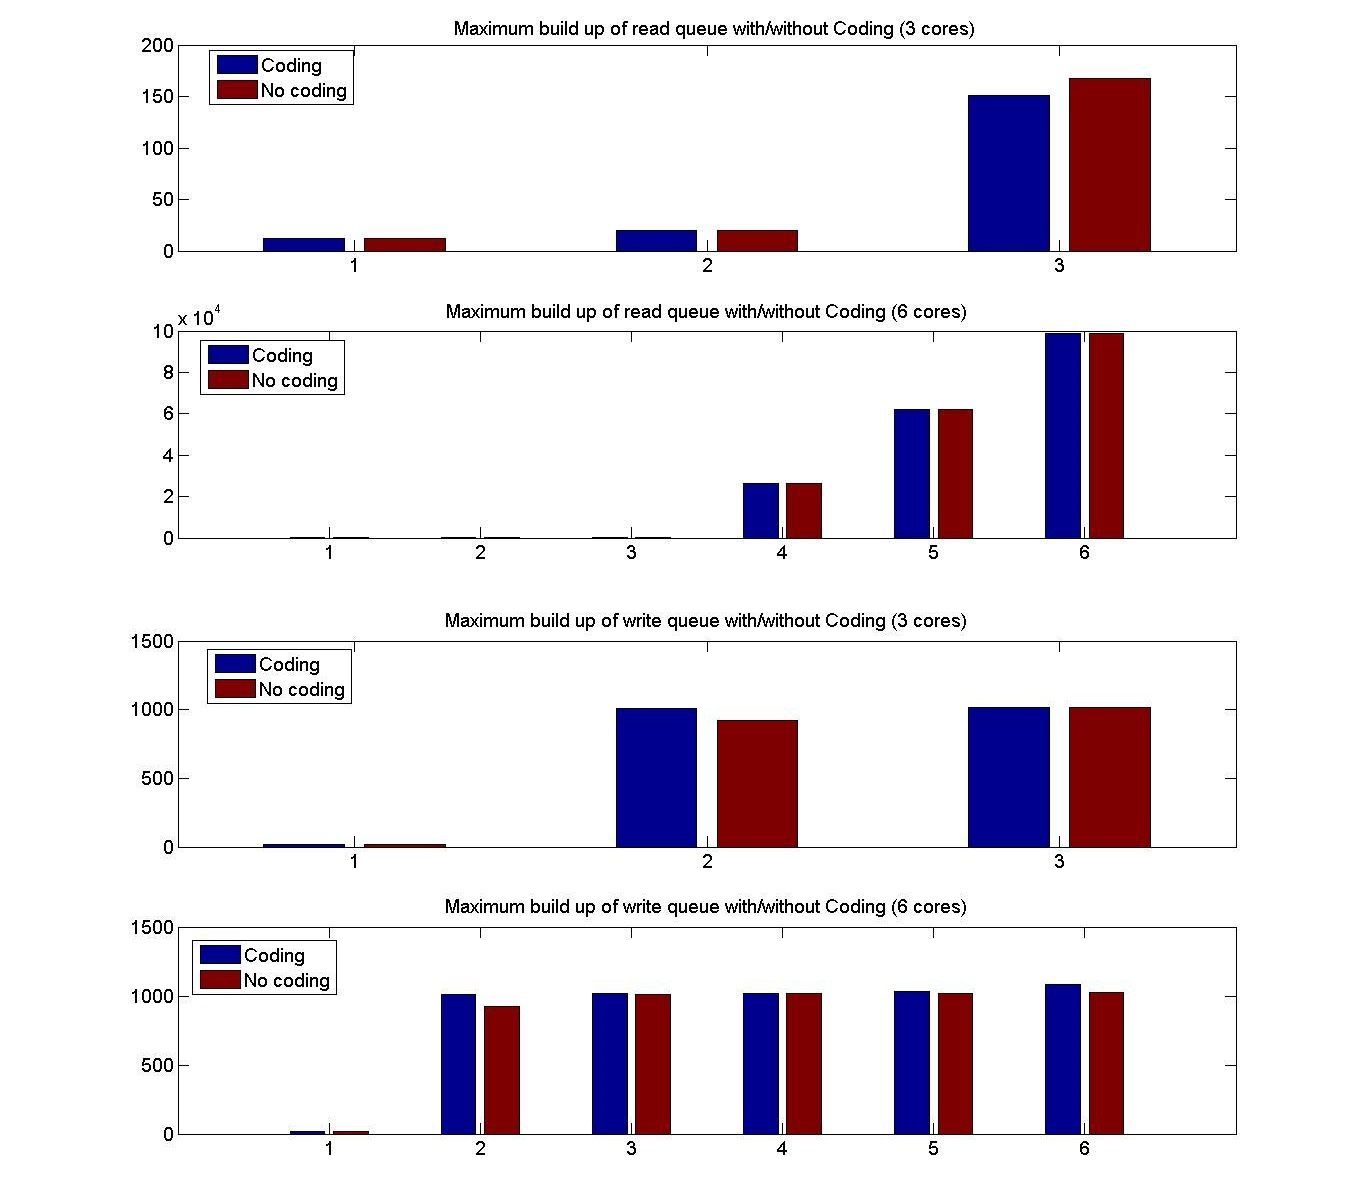
\includegraphics[width=150mm,natwidth=610,natheight=642]{fig/result_design2.jpg}
\caption{ Comparison of Design II with No coding case }
\label{fig:result_design2}
\end{figure}
}
\subsubsection{Code Scheme II}
\label{sec:design2}

Figure~\ref{fig:design2} illustrates the second code scheme explored in this paper. Again, the $8$ data banks $\{\mathbf{a}, \mathbf{b},\ldots, \mathbf{h}\}$ are partitioned into two groups containing $4$ data banks each. These two groups are then associated with two code regions. The first code region is similar to the previous code scheme, as it contains parity elements constructed from two data banks. The second code region contains data directly duplicated from single data banks. This code scheme further differs from the previous code scheme (cf. Figure~\ref{fig:design1}) in terms of the size and arrangement parity banks. Even though $L' = \alpha L$ rows from each data bank are stored in a coded manner by generating parity elements, the parity banks are assumed to be storing $2\alpha L > L'$ rows.

For a specific choice of $\alpha$, the storage overhead of this scheme is $20\alpha L$ which leads to a rate of $$\frac{8L}{8L + 20\alpha L} = \frac{2}{2 + 5\alpha}.$$ Note that this code scheme can support $5$ read accesses per data bank in a single memory clock cycle as opposed to $4$ read requests supported by the code scheme from Section~\ref{sec:design1}. However, this is made possible at the cost of extra storage overhead. Next, we discuss the performance of this code scheme in terms of the number of simultaneous read requests that can be served in the best and worst case.

%
%The second design, presented in figure 4, improves over first design by allowing 
%5 read accesses per bank per cycle. This design also divides banks into two 
%regions. The first region is
%Bank 1 to Bank 4 and 5 corresponding Parity banks. The two regions in figure 4 
%are upper 9 banks forming one region and lower 9 banks forming another. This 
%design allows intermix storage of parity among regions. The design uses 5 parity 
%banks per region. The data in this scheme is coded for both inter bank and 
%intra-bank. The intra-bank codes are stored in the alternate parity bank region. 
%This allows usage of parity banks from other region if they are available. \\
\begin{figure}[!ht]
%\centering
%\begin{minipage}[!t]{\linewidth}
	%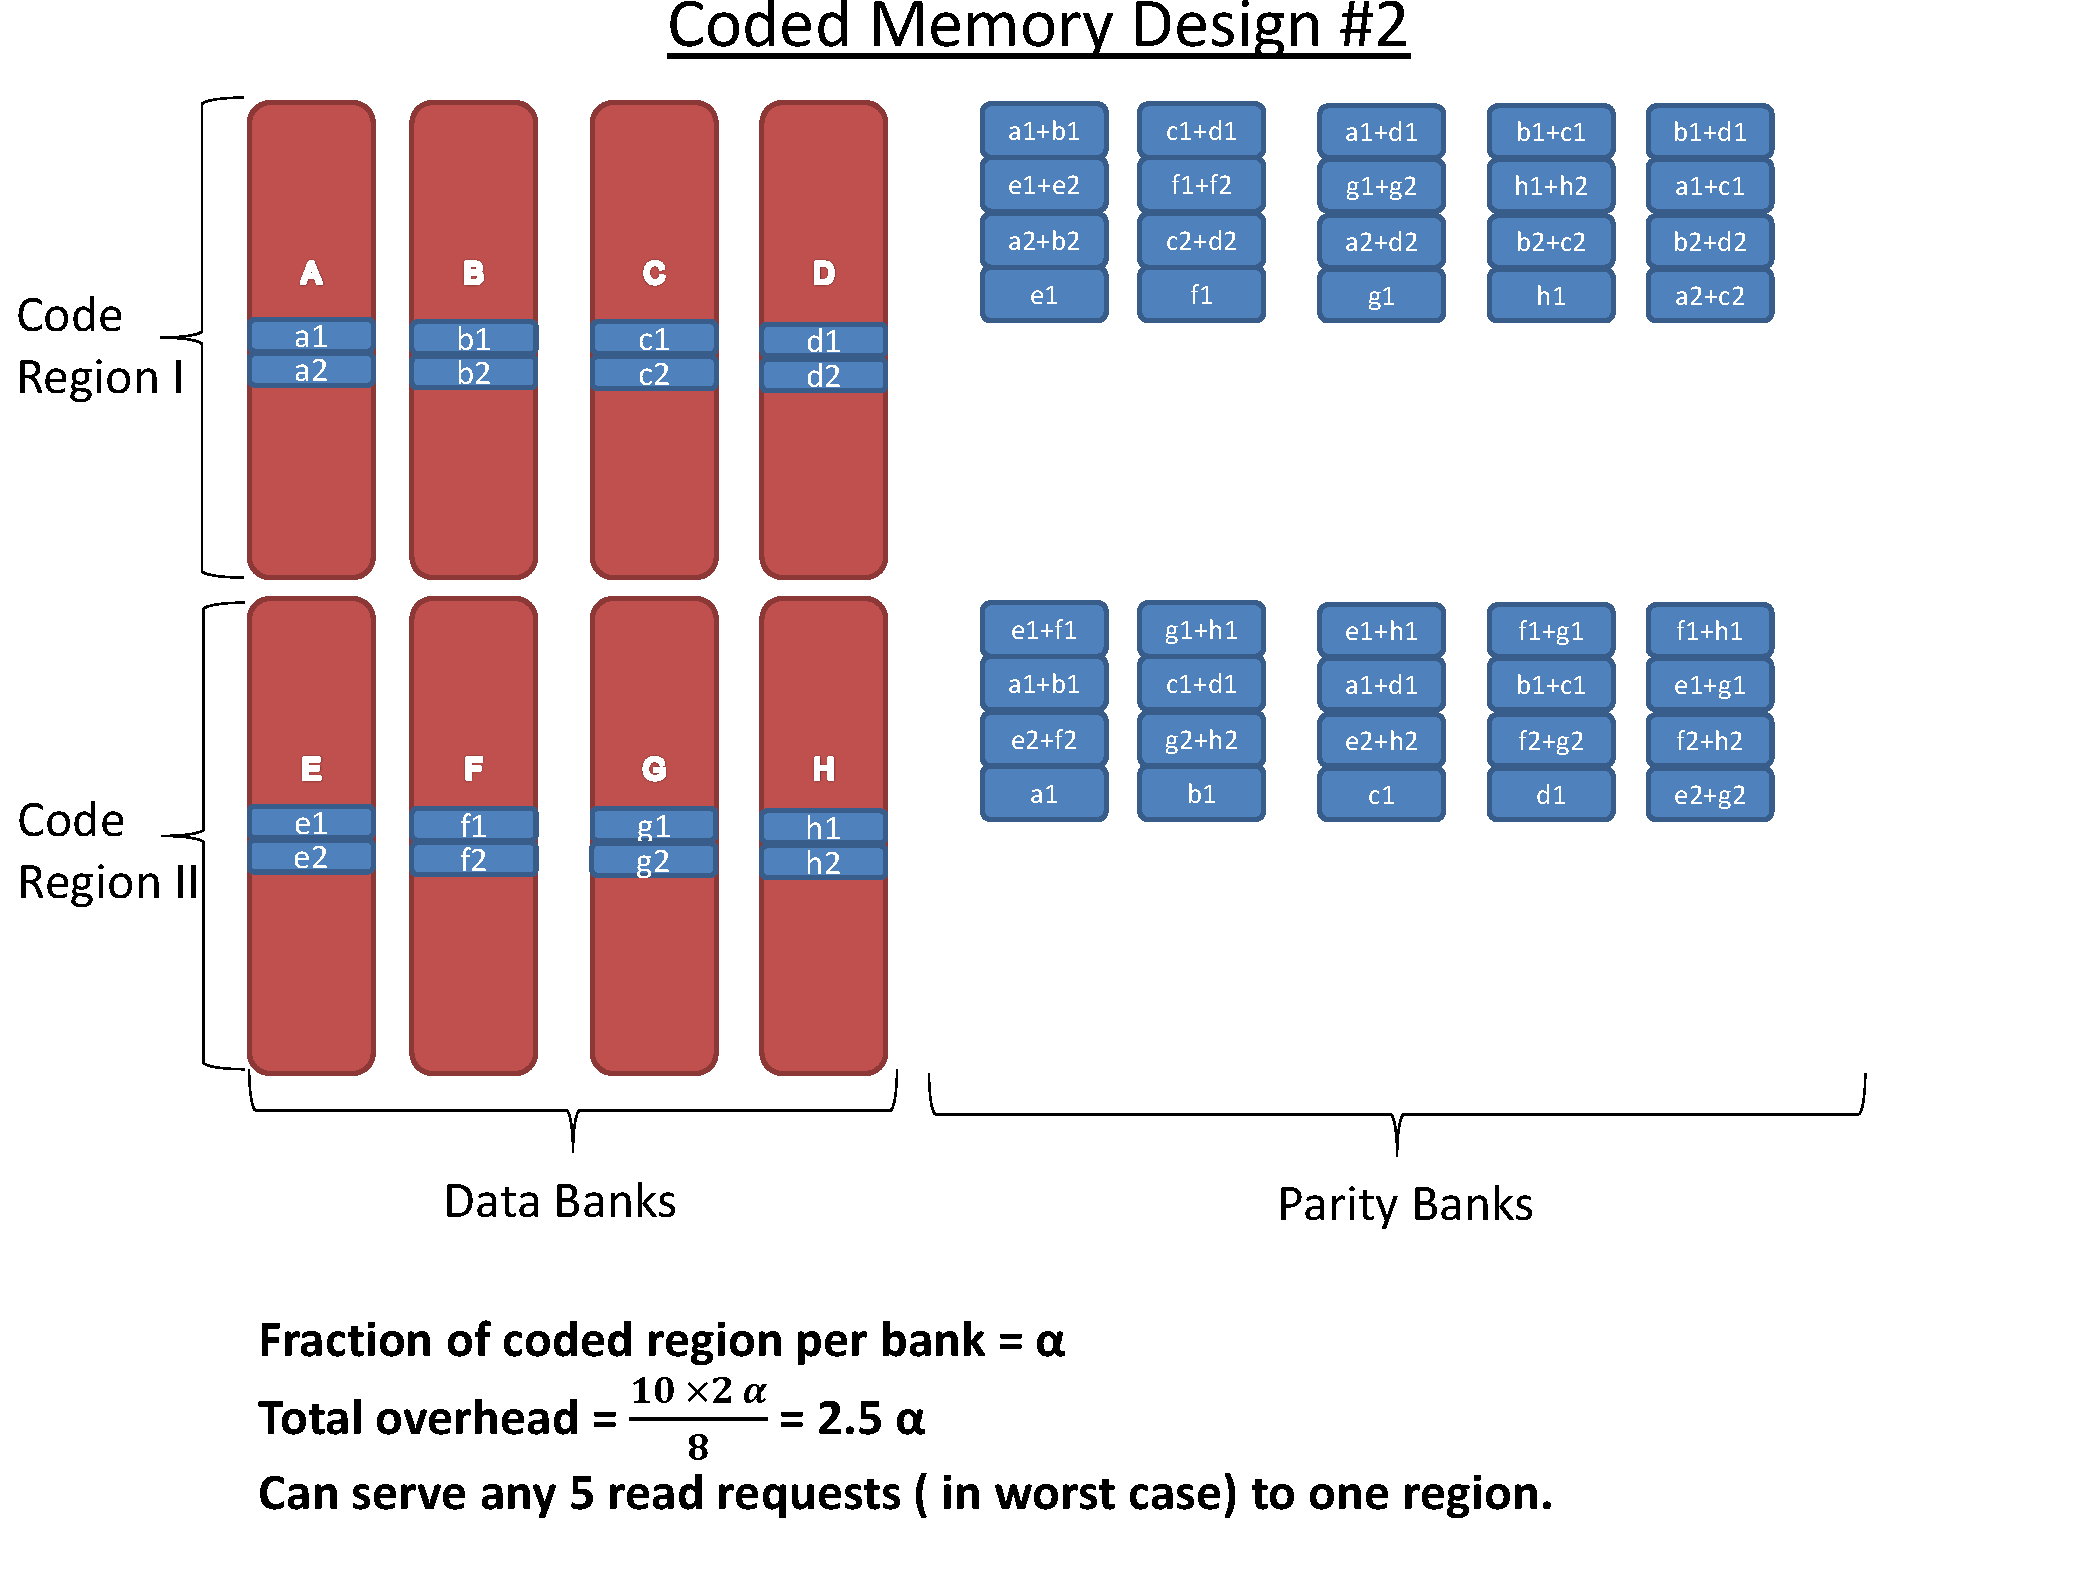
\includegraphics[width=1\linewidth]{fig/designII.pdf}
	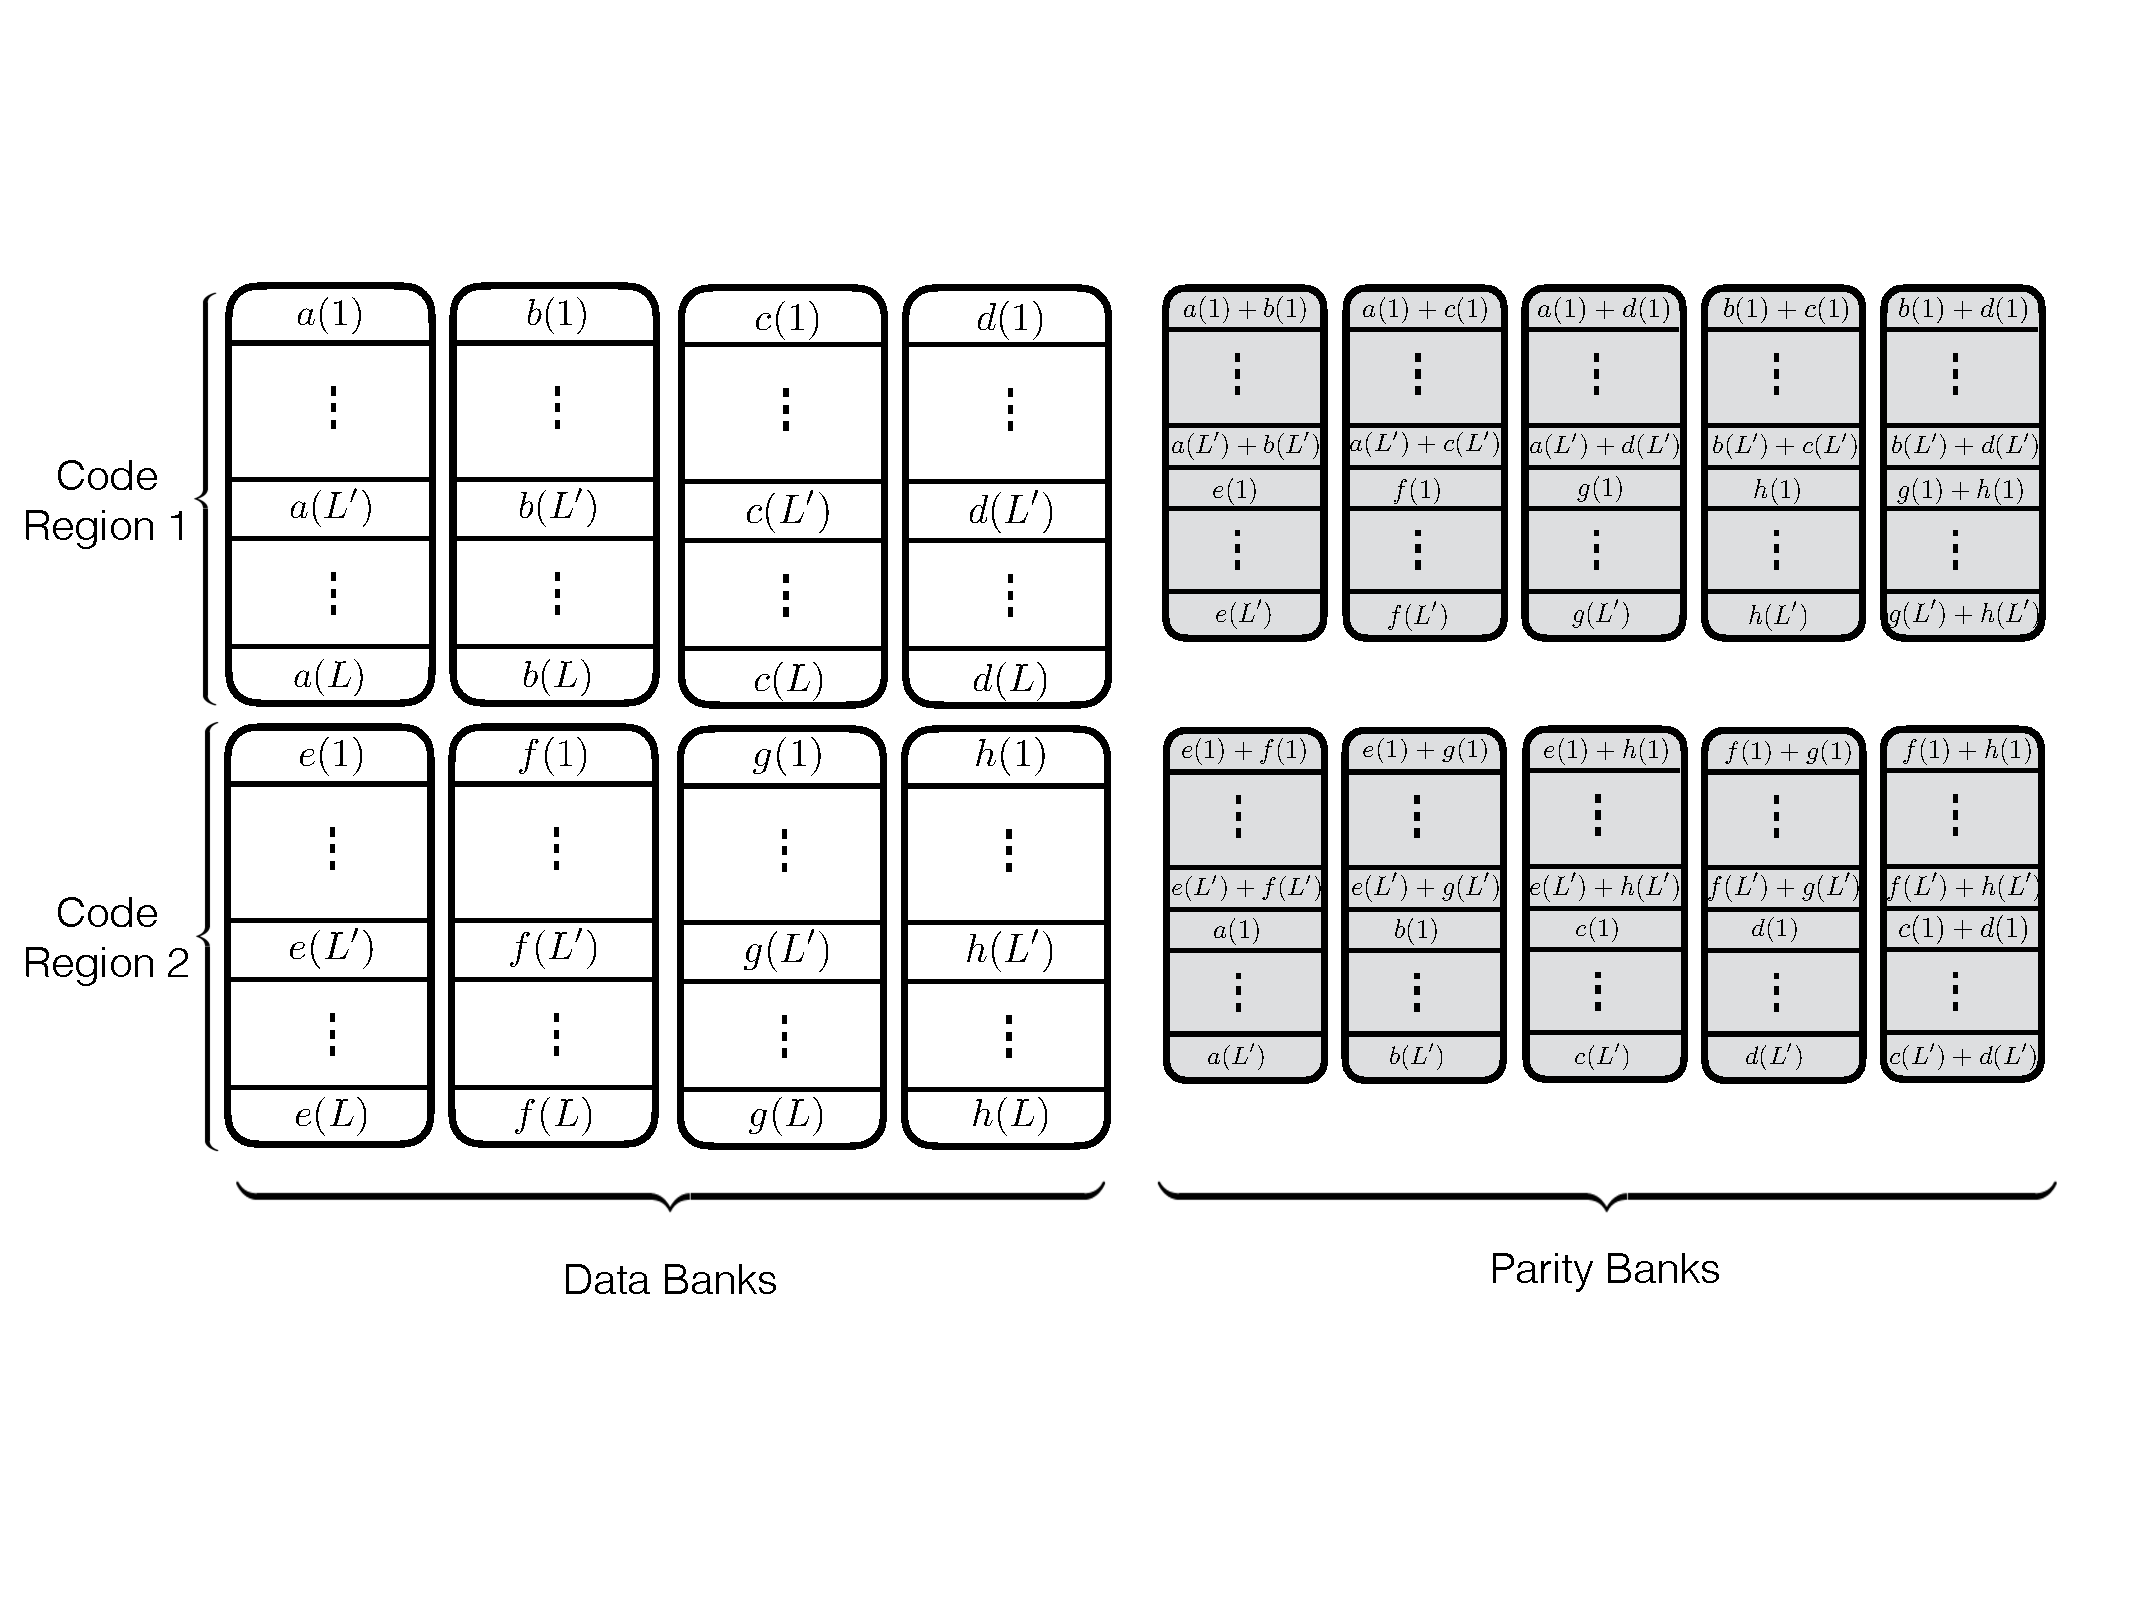
\includegraphics[width=1\linewidth]{fig/Code-Design-2.pdf}
	\caption{\it{Pictured here is an illustration of code scheme II.}}
	\label{fig:design2}
%\end{minipage}
\end{figure}

\noindent \textbf{Best case analysis:~} This code scheme achieves the best access performance when sequential accesses to the data banks are issued. In particular, this scheme can support up to $9$ read requests in a single memory clock cycle. Consider the scenario where we receive read requests for the following rows of the data banks. 
$$
\big\{a(1),b(1),c(1),d(1),a(2),b(2),c(2),d(2),a(3),b(3),c(3)\big\}
$$ Here, we can serve 
$\{a(1), b(1), c(1), d(1)\}$ using the data bank $\mathbf{a}$ with the parity banks storing the parity elements $\{a(1) + b(1),b(1)+c(1),c(1)+d(1)\}$. Similarly, we can serve the requests for the rows $\{a(2),b(2),d(2)\}$ using the data bank $\mathbf{b}$ with the parity banks storing the parity elements $\{a(2)+d(2), b(2)+d(2)\}$. Lastly, the request for the rows $c(2)$ and $d(3)$ is served using the data banks $\mathbf{c}$ and $\mathbf{d}$.\\


\noindent \textbf{Worst case analysis:~}The code scheme can enable $5$ simultaneous accesses in a single memory clock cycle in the
worst case. These are non-sequential and non-consecutive accesses to the memory banks. For 
example, when the access pattern corresponds to the rows $\{a(1),b(6),c(9),d(15),e(20)\}$, we can simultaneously serve 
these $5$ read requests with the help of our coded memory. In order to better utilize the unused banks in this case, we can use the prefetching 
mechanisms (cf. Section~\ref{sec:prefetching}) to look ahead in the queue and proactively download elements from the unused banks for future accesses.


% This design employs both inter-bank and intra-bank encoding in order to generate the content to be stored on the parity banks. In order to illustrate another flexibility that can be utilized while designing the storage space for a memory system, even though this code scheme encodes $\alpha L$ rows from each data bank, the parity banks are assumed to be storing $2\alpha L$ rows.


\subsubsection{Code Scheme III}
The next code scheme we discuss has locality 3, so each degraded read requires two parity banks to be served. This code scheme works with $9$ data bank $\{\mathbf{a}, \mathbf{b},\ldots, \mathbf{h}, \mathbf{z}\}$ and generates $9$ shallow parity banks. Figure~\ref{fig:design3} shows this scheme.
%The two designs discussed above achieve a rate of $2/5$. Here, we explore a code scheme which achieves a rate of $1/2$. 
%This design requires 9 data banks and 9 parity banks as shown in figure 5. It 
%also has a comparatively higher locality of 3. That is, it requires the memory 
%controller to "know" two out of three data elements to decode the third. 
The storage overhead of this scheme is $9\alpha L$ which corresponds to the rate of $\frac{1}{1 + \alpha}$. We note that this scheme possesses higher logical complexity as a result of its increased locality. 

This scheme supports $4$ simultaneous read access per bank per memory clock cycle as demonstrated by the following example. Suppose rows $\{a(1), a(2), a(3), a(4)\}$ are requested. $a(1)$ can be served directly from $\mathbf{a}$. $a(2)$ is served by means of a parity read and reads to banks $\mathbf{b}$ and $\mathbf{c}$, $a(3)$ is served by means of a parity read and reads to banks $\mathbf{d}$ and $\mathbf{g}$, and $a(4)$ is served by means of a parity read and reads to banks $\mathbf{e}$ and $\mathbf{z}$.

\noindent \textbf{Best case analysis:~} Following the analysis similar to Code Schemes I and II, the best case number of reads per cycle will be equal to the number of data and parity banks.

\noindent \textbf{Worst case analysis:~} Similar to coding schemes I and II, the number of reads per cycle is equal to the number of data banks. 
%The memory overhead here is less (just $\alpha$) compared to the previous designs. However, it possesses higher logical complexity because of increased locality. Example cases for this design are described below :
%\begin{itemize}
%
%	\item 4 reads for $a_0$: 1 read from $a_0$, 1 read from ($a_1$, $a_2$, 
%		$a_0$ + $a_1$ + $a_2$), 1 read from ($a_3$, $a_6$, $a_0$ + $a_3$ 
%		+ $a_6$), and the 4th read from ($a_4$, $a_8$, $a_0$ + $a_4$ + 
%		$a_8$).
%	\item 3 reads for $a_0$: 1 read from $a_0$, 1 read from ($a_3$, $a_6$, 
%		$a_0$ + $a_3$ + $a_6$), and the 3rd read from ($a_4$, $a_8$, 
%		$a_0$ + $a_4$ + $a_8$). \\
%	      1 read for $a_1$:  1 read from $a_1$.
%	\item 2 reads for $a_0$: 1 read from $a_0$ and the 2nd read from ($a_3$, 
%		$a_6$, $a_0$ + $a_3$ + $a_6$). \\
%	      2 reads for $a_1$: 1 read from $a_1$ and the 2nd read from ($a_4$, 
%	      $a_7$, $a_1$ + $a_4$ + $a_7$).
%	\item 2 reads for $a_0$: 1 read from $a_0$ and the 2nd read from ($a_3$, 
%		$a_6$, $a_0$ + $a_3$ + $a_6$). \\
%	      1 read for $a_1$: 1 read from $a_1$. \\
%	      1 read for $a_2$: 1 read from $a_2$.
%    \end{itemize}
%---------------------------------------
\begin{figure}[!ht]
	\centering
	\begin{minipage}[!t]{\linewidth}
		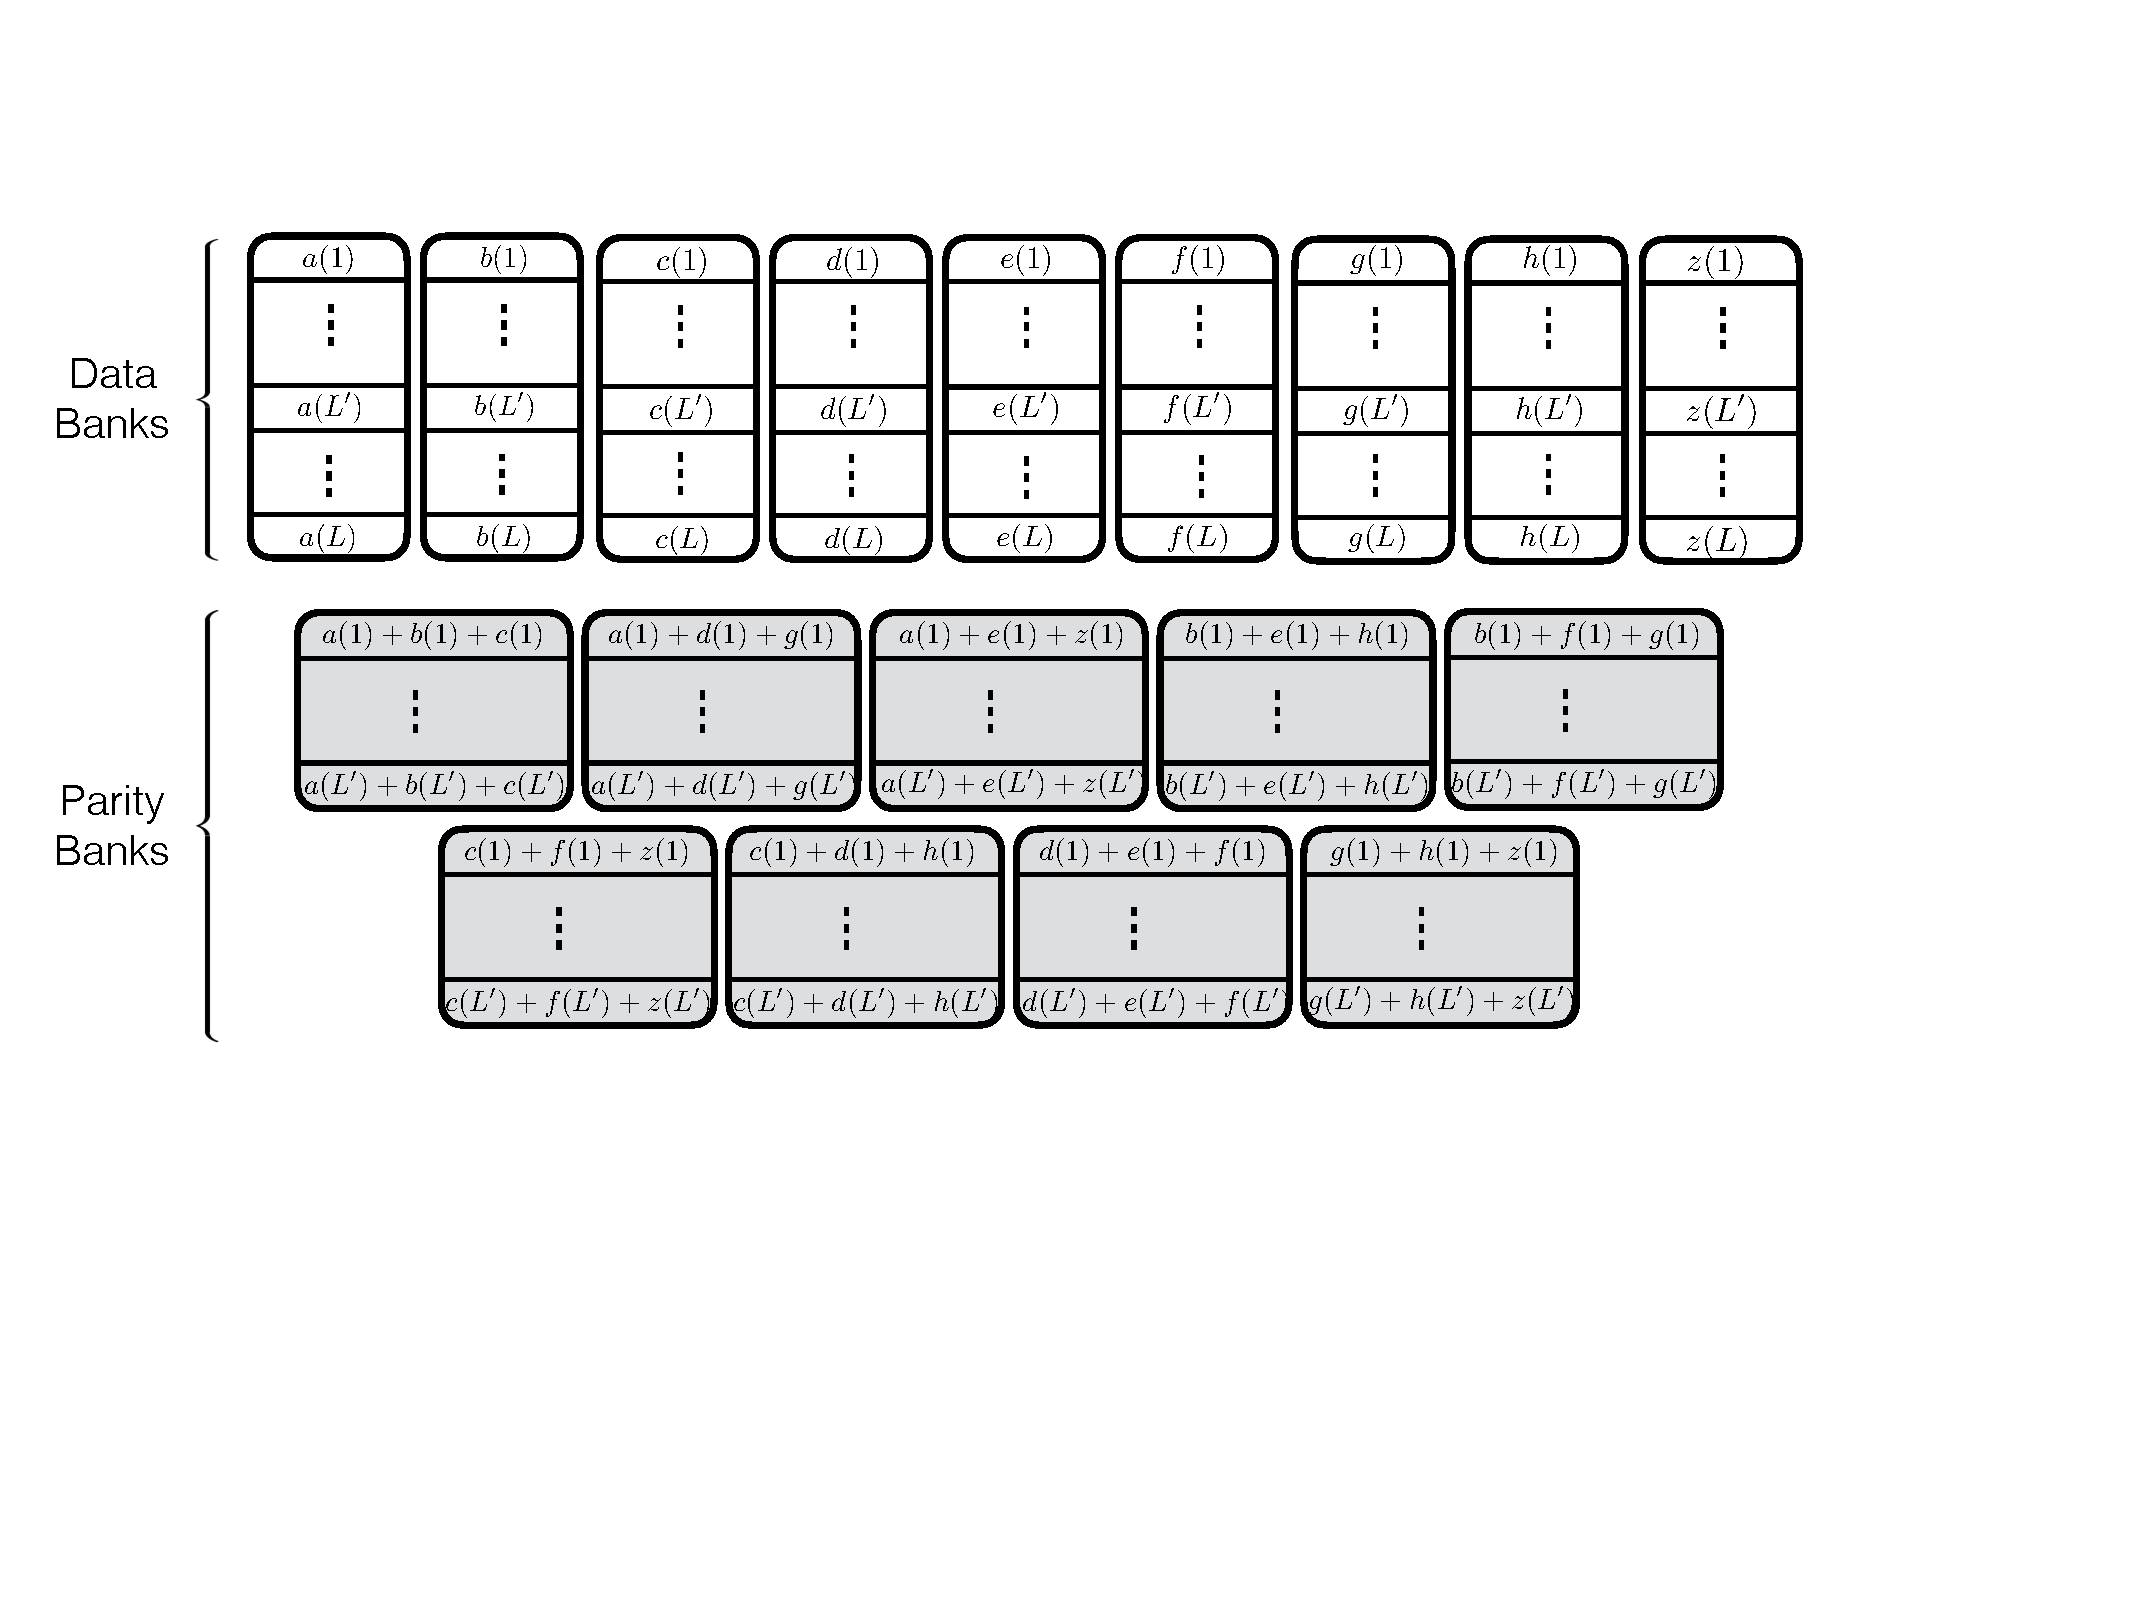
\includegraphics[width=\linewidth]{fig/Code-Design-3_9banks.pdf}
		\caption{\it{Pictured here is an illustration of code scheme III.}}
		\label{fig:design3}
	\end{minipage}
\end{figure}
%---------------------------------------

\begin{remark}
Note that the coding scheme in Figure~\ref{fig:design3} describes a system with $9$ data banks. However, we have set out to construct a memory system with $8$ data banks. It is straightforward to modify this code scheme to work with $8$ data banks $\{\mathbf{a}, \mathbf{b},\ldots, \mathbf{h}\}$ as shown in Figure~\ref{fig:design3_8}.
%Since most systems are implemented with number of banks as $2^n$ for some n. We present an 
%example of the code with 8 data banks in figure~\ref{fig:design3_8}. For using 8 data banks, 
%we drop the bank I. We also ignore the data from Bank I for constructing parity. So, three of 
%the parity banks have the locality of 2, while the rest of the parity banks have locality of 3.
% The new scheme for 8 data banks has 9 parity banks.
 \end{remark}
%---------------------------------------
\begin{figure}[!ht]
\centering
	\begin{minipage}[!t]{\linewidth}
		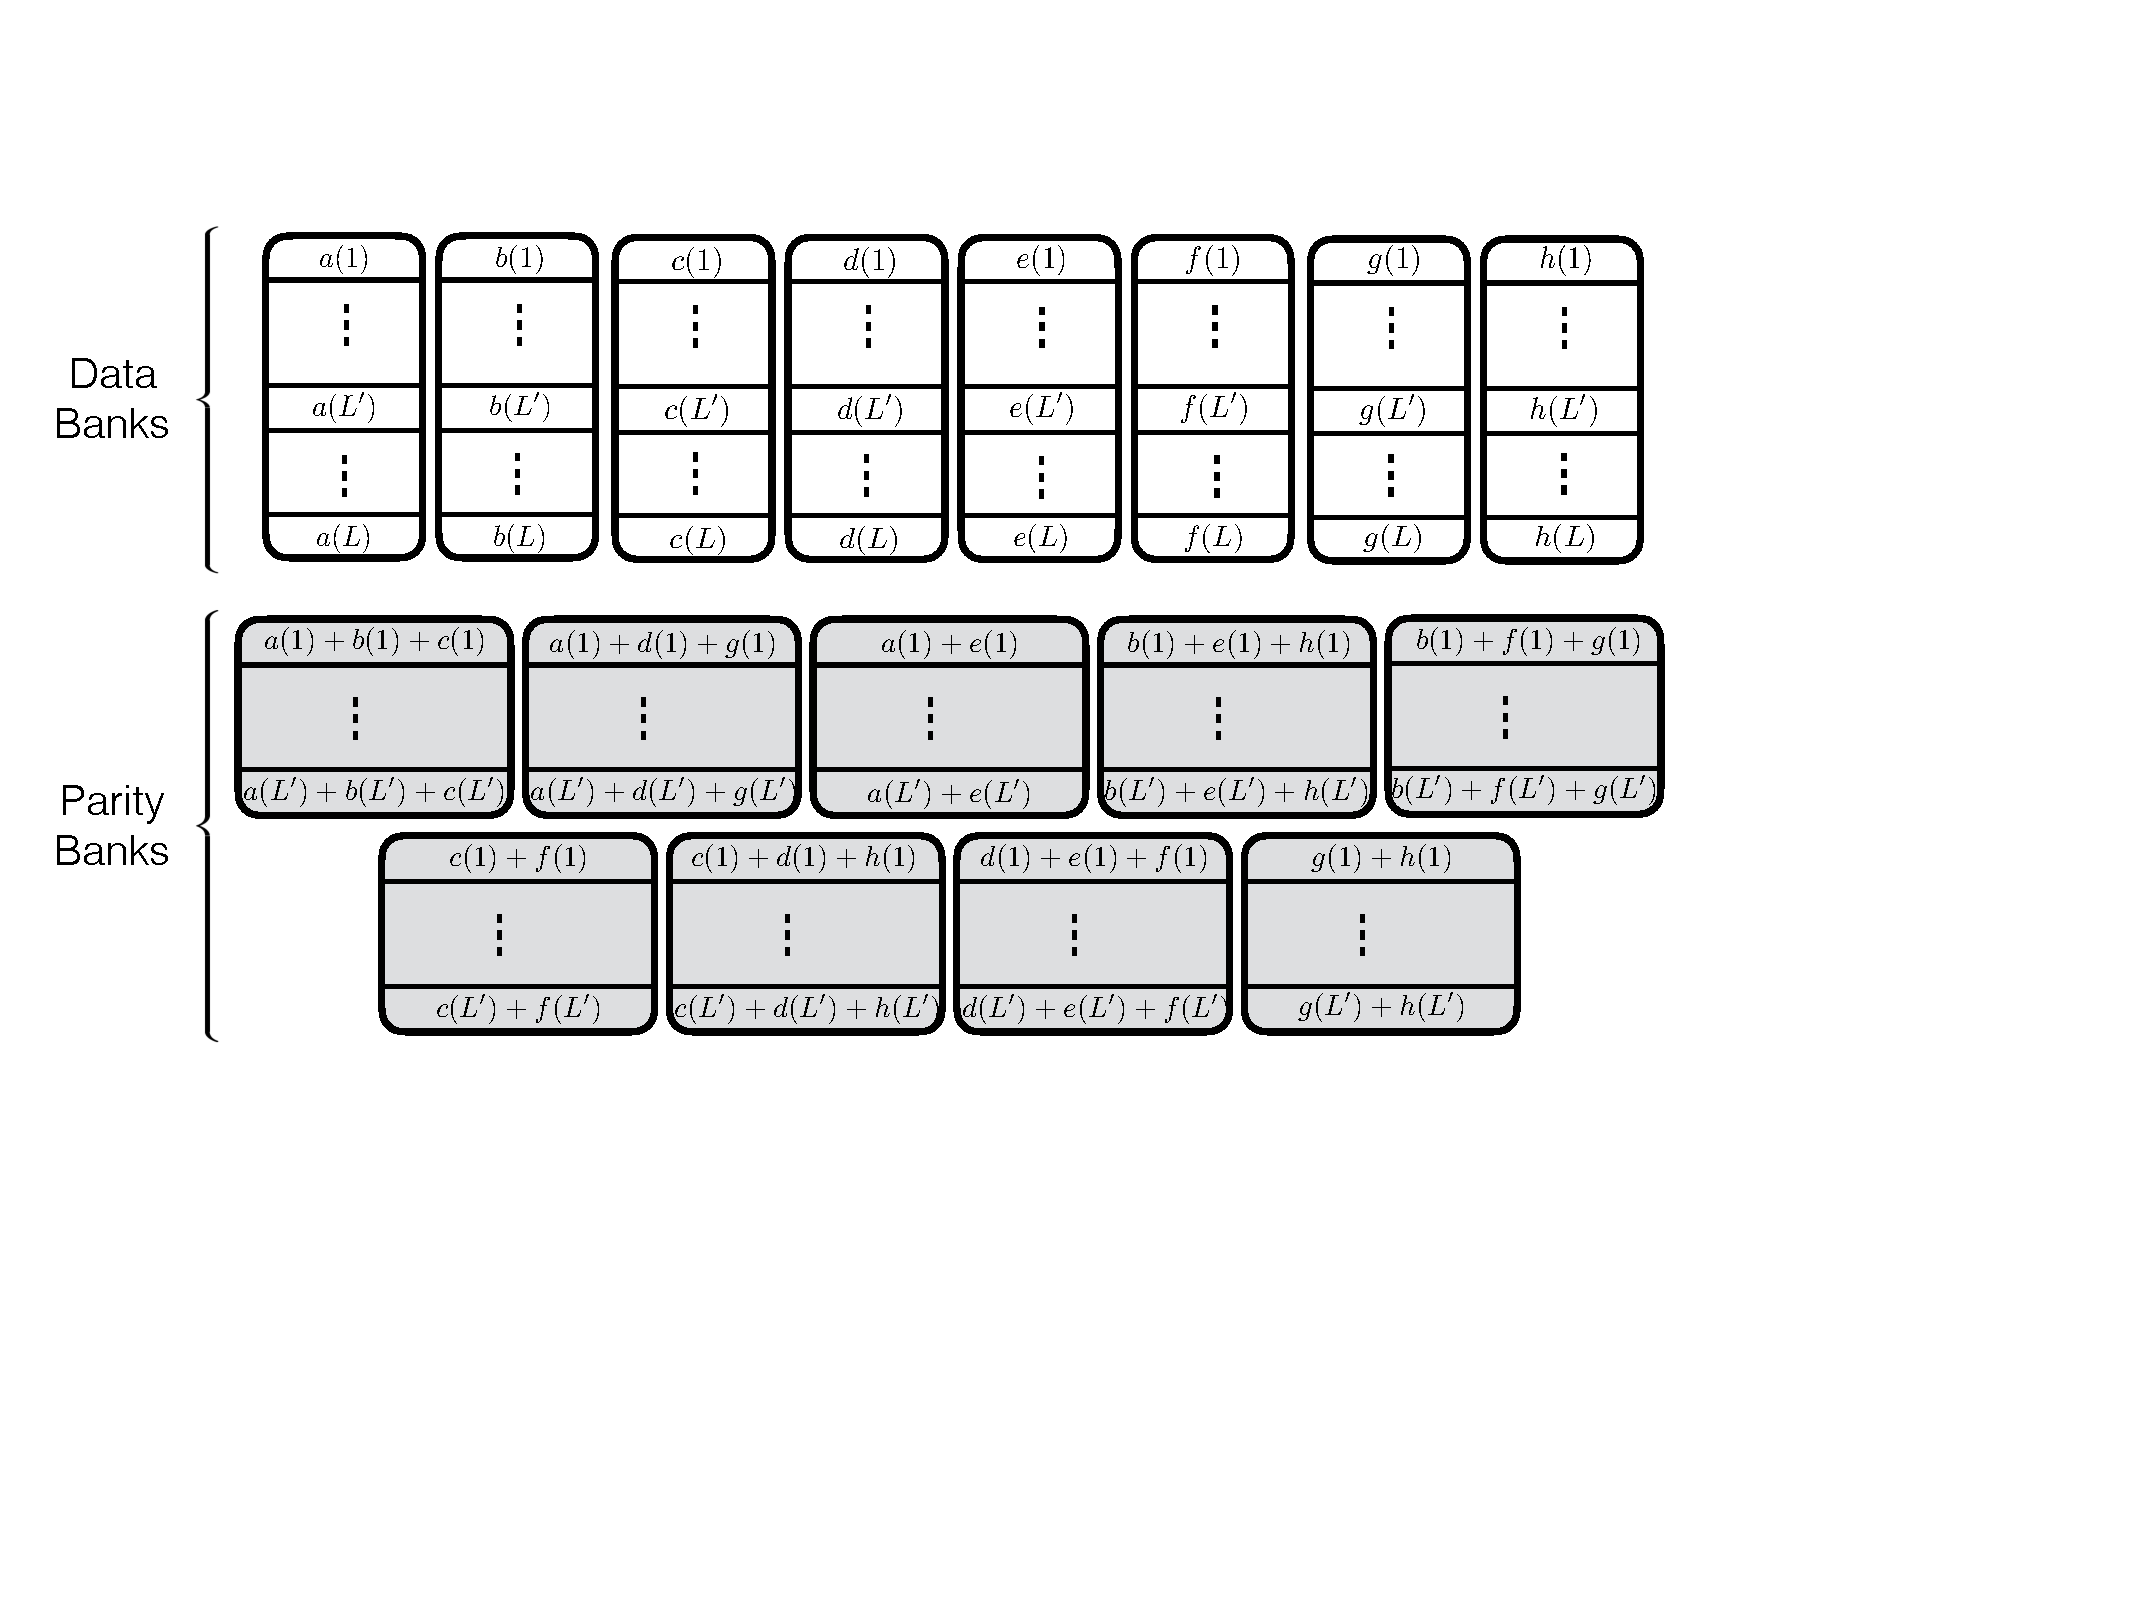
\includegraphics[width=\linewidth]{fig/Code-Design-3_8banks.pdf}
		\caption{\it{Pictured here is an illustration of code scheme III with 8 data banks.}}
		\label{fig:design3_8}
	\end{minipage}
\end{figure}
%---------------------------------------

\begin{comment}
Since the locality is 3 here in this design, i.e. , each parity is made up of combination of 3 data banks, we need to make sure that all three requests are in one line to be able to use the parity bank. 
For example parity bank 0 contains A+B+C. So, the following scenarios arise:
\begin{itemize}
	\item {\em Scenario I}: 1st request of A and 1st request of B are in same row. Then, we can search for a request in the same row for bank C by doing a look ahead. 
	\item {\em Scenario II}: 1st request of A and 1st request of C are in same row. Then, we can search for a request in the same row for bank B by doing a look ahead. 
	\item {\em Scenario III}: 1st request of B and 1st request of C are in same row. Then, we can search for a request in the same row for bank A by doing a look ahead. 
\end{itemize}
So, the simple pseudo code for doing this would be :\\
\begin{verbatim}
for each data bank 
    for each auxiliary bank1 of data bank
            Look ahead in auxiliary bank2 and check if 3 request in a row.
        end
    end
\end{verbatim}
Example: - \\
For {\bf data bank} to be {\bf A} \\
{\bf auxiliary bank1} goes from [B C D G A E] \\
{\bf auxiliary bank2} goes from [C B G D E A] \\
  The element A is just there in {\bf auxiliary bank1} and {\bf auxiliary bank2} to maintain the symmetry because A + E has locality of 2.
\end{comment}
